%==============================================================
%  Báo cáo môn học — Chuyên đề nghiên cứu 1
%  Đề tài: Tìm hiểu điện toán lượng tử cơ bản
%          và bài toán biên dịch mạch lượng tử
%
%  HOW TO COMPILE (Overleaf or local):
%   Requires LuaLaTeX (Vietnamese Unicode text + fontspec).
%   latexmk   — latexmk -pdflua -interaction=nonstopmode -outdir=build report.tex
%   Overleaf  — Menu > Compiler > LuaLaTeX
%
%  Cấu trúc:
%   report.tex            preamble, trang bìa, tóm tắt, mục lục
%   sections/*.tex        nội dung từng chương
%   imgs/                 logo trường
%==============================================================
\documentclass[11pt,a4paper]{article}

% ---- Layout -------------------------------------------------
\usepackage[top=1in,bottom=1in,left=1.1in,right=1.1in]{geometry}
\usepackage{setspace}
\setstretch{1.15}

% ---- Core packages ------------------------------------------
\usepackage{fontspec}
\setmainfont{lmroman10}[
  Extension = .otf,
  UprightFont = *-regular,
  BoldFont = *-bold,
  ItalicFont = *-italic,
  BoldItalicFont = *-bolditalic,
]
\setmonofont{lmmono10}[
  Extension = .otf,
  UprightFont = *-regular,
  ItalicFont = *-italic,
  BoldFont = lmmonolt10-bold,
  Scale = 0.95,
]
\usepackage{amsmath,amssymb,amsthm}
\usepackage{braket}
\usepackage{booktabs}
\usepackage{multirow}
\usepackage{array}
\usepackage{tabularx}
\usepackage{graphicx}
\graphicspath{{imgs/}{./imgs/}}
\usepackage{xcolor}
\usepackage{hyperref}
\usepackage{caption}
\usepackage{subcaption}
\usepackage{tikz}
\usetikzlibrary{arrows.meta, positioning, shapes.geometric, calc, quantikz2}
\usepackage{pgfplots}
\pgfplotsset{compat=1.18}
\usepackage{enumitem}
\usepackage{parskip}
\usepackage{listings}
\usepackage{algorithm}
\usepackage{algpseudocode}
\usepackage[most]{tcolorbox}

% ---- Colors (mirrored from cv-report) -----------------------
\definecolor{ProbRed}{HTML}{C0392B}
\definecolor{OkGreen}{HTML}{1E8449}
\definecolor{AccentBlue}{HTML}{2C6FBB}
\definecolor{OrangeYellow}{HTML}{D4890B}
\definecolor{Purple}{HTML}{8E44AD}
\definecolor{CodeBg}{HTML}{F5F7FA}

% ---- TikZ styles --------------------------------------------
\tikzset{
  box/.style={rectangle, rounded corners, draw=#1, thick, fill=#1!10,
              minimum width=2.4cm, minimum height=0.7cm,
              font=\small, align=center},
  box/.default=AccentBlue,
  arr/.style={-{Stealth[length=2mm]}, thick},
}

% ---- Hyperref setup -----------------------------------------
\hypersetup{
  colorlinks=true,
  linkcolor=AccentBlue,
  citecolor=AccentBlue,
  urlcolor=AccentBlue,
  pdftitle={Điện toán lượng tử cơ bản và biên dịch mạch lượng tử},
  pdfauthor={Nguyễn Tất Chung},
}

% ---- Vietnamese names for floats / sections -----------------
\renewcommand{\contentsname}{Mục lục}
\renewcommand{\abstractname}{Tóm tắt}
\renewcommand{\figurename}{Hình}
\renewcommand{\tablename}{Bảng}
\renewcommand{\refname}{Tài liệu tham khảo}
\renewcommand{\listfigurename}{Danh sách hình vẽ}
\renewcommand{\listtablename}{Danh sách bảng}
\renewcommand{\lstlistingname}{Đoạn mã}
\floatname{algorithm}{Thuật toán}
\renewcommand{\algorithmicrequire}{\textbf{Đầu vào:}}
\renewcommand{\algorithmicensure}{\textbf{Đầu ra:}}

\theoremstyle{definition}
\newtheorem{definition}{Định nghĩa}[section]
\newtheorem{theorem}{Định lý}[section]
\newtheorem{example}{Ví dụ}[section]

% ---- Code listings (Python / Qiskit) ------------------------
\lstset{
  language=Python,
  basicstyle=\ttfamily\small,
  keywordstyle=\color{AccentBlue},
  commentstyle=\color{OkGreen}\itshape,
  stringstyle=\color{ProbRed},
  backgroundcolor=\color{CodeBg},
  frame=single, rulecolor=\color{black!15},
  breaklines=true, columns=fullflexible, keepspaces=true,
  showstringspaces=false, xleftmargin=4pt, xrightmargin=4pt,
  aboveskip=6pt, belowskip=6pt,
}

% ---- Callout boxes ------------------------------------------
\newtcolorbox{keybox}[1][Ghi nhớ]{
  enhanced, breakable, colback=AccentBlue!6, colframe=AccentBlue,
  fonttitle=\bfseries\small, title=#1, boxrule=0.6pt, arc=2pt,
  left=6pt, right=6pt, top=4pt, bottom=4pt}
\newtcolorbox{warnbox}[1][Lưu ý]{
  enhanced, breakable, colback=ProbRed!5, colframe=ProbRed,
  fonttitle=\bfseries\small, title=#1, boxrule=0.6pt, arc=2pt,
  left=6pt, right=6pt, top=4pt, bottom=4pt}

% ---- Shorthands ---------------------------------------------
\newcommand{\code}[1]{\texttt{#1}}
\newcommand{\cx}{\code{cx}}
\newcommand{\Tr}{\mathrm{Tr}}

% ---- Title (metadata only; cover page below is custom) -------
\title{Tìm hiểu điện toán lượng tử cơ bản và bài toán biên dịch mạch lượng tử}
\author{Nguyễn Tất Chung}
\date{\today}

\begin{document}

%==============================================================
% Trang bìa (theo mẫu Trường Đại học Phenikaa)
%==============================================================
\begin{titlepage}
\thispagestyle{empty}
\setlength{\fboxsep}{1cm}
\setlength{\fboxrule}{0.6pt}
\noindent\fbox{%
  \begin{minipage}[c][\dimexpr\textheight-2\fboxsep-2\fboxrule\relax][c]{\dimexpr\textwidth-2\fboxsep-2\fboxrule\relax}
  \begin{center}
    {\bfseries BỘ GIÁO DỤC VÀ ĐÀO TẠO}\\
    {\bfseries TRƯỜNG ĐẠI HỌC PHENIKAA}\\[2pt]
    \rule{3.5cm}{0.4pt}

    \vfill

    
\includegraphics[width=0.55\linewidth]{phenikaa-uni-symbol.png}

    \vfill

    {\LARGE\bfseries BÁO CÁO MÔN HỌC}

    \vspace{2.5em}

    {\Large\bfseries TÊN ĐỀ TÀI:}\\[0.8em]
    {\large\bfseries TÌM HIỂU ĐIỆN TOÁN LƯỢNG TỬ CƠ BẢN\\
    VÀ BÀI TOÁN BIÊN DỊCH MẠCH LƯỢNG TỬ}\\[0.6em]
    {\normalsize\itshape Fundamentals of Quantum Computing\\
    and Quantum Circuit Compilation}

    \vfill

    \begin{tabular}{@{}l@{}}
      Học phần: \quad Chuyên đề nghiên cứu 1\\
      % Bậc đào tạo: \quad Cao học (Thạc sĩ)
    \end{tabular}

    \vspace{2em}

    \begin{tabular}{@{}ll@{}}
      Học viên thực hiện: & Nguyễn Tất Chung \\[0.3em]
      Giảng viên hướng dẫn: & Phạm Văn Cảnh \\
                            & Nguyễn Văn Duy
    \end{tabular}

    \vfill

    {\bfseries Hà Nội, tháng 10 năm 2026}
  \end{center}
  \end{minipage}%
}
\end{titlepage}

%==============================================================
\begin{abstract}
Máy tính lượng tử hứa hẹn giải một số bài toán nhanh hơn máy tính cổ điển, nhưng các thiết bị
hiện nay (thời kỳ \emph{NISQ} -- Noisy Intermediate-Scale Quantum) chỉ hỗ trợ một tập cổng nhỏ,
chỉ cho phép cổng hai qubit giữa những cặp qubit kề nhau, và mọi cổng đều có sai số. Khoảng cách
giữa mạch lý tưởng mà người lập trình viết và mạch thực sự chạy trên phần cứng được lấp đầy bởi
\textbf{quantum compiler} (trong Qiskit gọi là \emph{transpiler}). Báo cáo này trình bày một lộ
trình tự học có hệ thống, đi từ nền tảng tới bài toán nghiên cứu: (i) qubit, ký hiệu Dirac (ket),
superposition, phép đo và entanglement; (ii) các cổng lượng tử một và nhiều qubit; (iii) các thuật
toán lượng tử cơ bản xây dựng trên cơ chế \emph{phase kickback} -- Deutsch--Jozsa,
Bernstein--Vazirani, Grover -- cùng teleportation và superdense coding; (iv) quá trình biên dịch mạch
gồm layout, routing, synthesis và tối ưu, được nhìn như một \textbf{bài toán tối ưu}. Phần cuối
phát biểu qubit routing thành một Markov decision process, hiện thực thành môi trường
\code{gymnasium} có kiểm tra tính đúng đắn, và dựng một thang mốc so sánh trung thực. Các thực
nghiệm với Qiskit~2.5 cho thấy compiler ảnh hưởng mạnh tới chất lượng mạch: topology quyết định số
SWAP (75 trên \emph{line} so với 25 trên \emph{grid} cho cùng mạch 9 qubit), layout tốt giảm
16\% số SWAP, thuật toán \emph{gridsynth} cần ít cổng $T$ hơn Solovay--Kitaev hơn 7 lần, và một
policy tham lam đơn giản vẫn kém \code{SabreSwap} 25\% -- khoảng trống mà các phương pháp
reinforcement learning trong Chuyên đề nghiên cứu 2 sẽ nhắm tới.

\medskip
\noindent\textbf{Từ khoá:} quantum computing, qubit, quantum gate, quantum algorithm, quantum
circuit compilation, transpiler, qubit routing, SABRE, T-count, reinforcement learning, Qiskit.
\end{abstract}

\tableofcontents
\newpage

%==============================================================
\section{Mở đầu}
\label{sec:intro}
%==============================================================

\subsection{Bối cảnh}

Điện toán lượng tử (quantum computing) là mô hình tính toán dựa trên các nguyên lý của cơ học lượng
tử: \emph{superposition}, \emph{entanglement} và \emph{interference}. Thay vì bit cổ điển chỉ nhận
giá trị $0$ hoặc $1$, đơn vị thông tin của máy tính lượng tử là \textbf{qubit} -- một vector đơn vị
trong không gian Hilbert hai chiều. Một hệ $n$ qubit được mô tả bởi $2^n$ amplitude phức, và các
thuật toán lượng tử khai thác cấu trúc này để giải một số bài toán với số bước ít hơn đáng kể so với
mọi thuật toán cổ điển đã biết: Grover tìm kiếm trong $O(\sqrt{N})$ bước thay vì $O(N)$
\cite{grover1996}, Shor phân tích thừa số nguyên tố trong thời gian đa thức \cite{shor1997}.

Tuy nhiên, các máy tính lượng tử hiện nay thuộc thời kỳ \textbf{NISQ} (Noisy Intermediate-Scale
Quantum) \cite{preskill2018nisq}: vài chục tới vài trăm qubit, chưa có sửa lỗi đầy đủ, và mỗi phép
toán đều có sai số. Cụ thể, một thiết bị thật áp đặt ba ràng buộc lên mạch lượng tử:
\begin{enumerate}[noitemsep]
  \item \textbf{Basis gates} -- chỉ thực hiện được một tập cổng nhỏ, ví dụ
    $\{\code{rz}, \code{sx}, \code{x}, \code{cx}\}$.
  \item \textbf{Connectivity} -- cổng hai qubit chỉ thực hiện được trên các cặp qubit nối trực tiếp
    với nhau theo một đồ thị cố định (\emph{coupling map}).
  \item \textbf{Noise} -- cổng hai qubit có xác suất lỗi khoảng $10^{-3}$--$10^{-2}$, tệ hơn cổng
    một qubit một tới hai bậc.
\end{enumerate}

Người lập trình viết mạch ở mức trừu tượng (dùng Toffoli, SWAP, cổng giữa hai qubit bất kỳ), còn
thiết bị chỉ chạy được mạch thoả cả ba ràng buộc trên. Bước dịch mạch lý tưởng thành mạch chạy được
gọi là \textbf{quantum circuit compilation} -- trong Qiskit gọi là \textbf{transpilation}. Hình
\ref{fig:motivation} minh hoạ mức độ chênh lệch: một mạch 5 qubit có độ sâu (\emph{depth}) 6 sau khi
biên dịch lên một thiết bị có coupling map dạng đường thẳng trở thành mạch có depth 40 với 19 cổng
\cx{}. Toàn bộ khoảng cách đó do compiler quyết định, và mỗi cổng \cx{} tiết kiệm được là một phần
sai số bớt đi.

\begin{figure}[h]
  \centering
  \begin{tikzpicture}[node distance=1.2cm]
    \node[box=AccentBlue, minimum width=3.4cm, minimum height=1.6cm] (src)
      {\textbf{Mạch lý tưởng}\\ depth 6, size 11\\ \code{ccx}, \code{swap}, \code{cz}, \code{ry}};
    \node[box=Purple, right=1.4cm of src, minimum width=2.8cm, minimum height=1.6cm] (tr)
      {\textbf{Transpiler}\\ layout, routing,\\ synthesis, tối ưu};
    \node[box=ProbRed, right=1.4cm of tr, minimum width=3.4cm, minimum height=1.6cm] (dst)
      {\textbf{Mạch chạy được}\\ depth 40, size 65\\ 19 \code{cx}, 27 \code{rz}, 12 \code{sx}};
    \draw[arr] (src) -- (tr);
    \draw[arr] (tr) -- (dst);
    \node[below=0.25cm of tr, font=\footnotesize, align=center, text=black!70]
      {basis $\{\code{cx},\code{rz},\code{sx},\code{x}\}$, coupling map \code{line(5)}};
  \end{tikzpicture}
  \caption{Cùng một thuật toán, mạch thật sự chạy trên thiết bị lớn hơn mạch được viết rất nhiều
  (số liệu đo trong notebook \code{02\_compilation/00}, Qiskit 2.5.2, \code{optimization\_level=2}).}
  \label{fig:motivation}
\end{figure}

Vì phần lớn các bài toán con của compilation (chọn layout, chèn SWAP tối thiểu, tổng hợp cổng tối
ưu) đều là NP-hard \cite{siraichi2018allocation}, các compiler thực tế dùng \emph{heuristic} do con
người thiết kế, tiêu biểu là thuật toán SABRE \cite{li2019sabre}. Điều này mở ra một hướng nghiên cứu
đang phát triển mạnh: dùng \textbf{reinforcement learning} (RL) để học các quyết định biên dịch tốt
hơn heuristic \cite{pozzi2022rlrouting, fosel2021rlopt, ruiz2025alphatensor, riu2025zx}.

\subsection{Mục tiêu của chuyên đề}

Chuyên đề nghiên cứu 1 đặt mục tiêu xây dựng nền tảng đủ vững để bắt đầu nghiên cứu về biên dịch mạch
lượng tử, cụ thể:
\begin{enumerate}[noitemsep]
  \item Nắm vững các khái niệm cơ bản: qubit, ký hiệu Dirac (ket/bra), superposition, phép đo,
    entanglement.
  \item Hiểu các cổng lượng tử một và nhiều qubit dưới dạng ma trận unitary, và cách chúng tạo nên
    mạch lượng tử.
  \item Hiểu cơ chế chung của các thuật toán lượng tử cơ bản (phase kickback, interference) qua
    Deutsch--Jozsa, Bernstein--Vazirani, Grover, teleportation và superdense coding.
  \item Phân tích quá trình biên dịch mạch trong Qiskit như một \textbf{bài toán tối ưu}: các stage,
    cấu trúc dữ liệu, hàm cost, và các thuật toán layout, routing, synthesis.
  \item Phát biểu qubit routing thành một Markov decision process (MDP), hiện thực thành môi trường
    \code{gymnasium} \textbf{đúng semantics}, và dựng \textbf{baseline trung thực} để làm nền cho
    các thí nghiệm RL ở Chuyên đề nghiên cứu 2.
\end{enumerate}

\subsection{Phạm vi và công cụ}

Báo cáo giới hạn ở mô hình mạch lượng tử (quantum circuit model) và các thiết bị dạng cổng
(gate-based). Mọi thí nghiệm được thực hiện bằng \textbf{Qiskit 2.5} \cite{qiskit2024} và
\code{qiskit-aer} trên simulator, với \code{gymnasium} cho môi trường RL. Toàn bộ mã nguồn được tổ
chức thành một chuỗi Jupyter notebook trong kho mã \code{master-research-1}, chia làm ba phần tương
ứng với các chương của báo cáo (Phụ lục~B). Mọi con số trong báo cáo đều tái lập được
bằng notebook tương ứng.

\subsection{Cấu trúc báo cáo}

Báo cáo đi theo trình tự \emph{ket $\to$ cổng $\to$ thuật toán $\to$ compilation}, mỗi chương là nền
cho chương sau:
\begin{itemize}[noitemsep]
  \item \textbf{Mục~\ref{sec:basics}} trình bày qubit, ký hiệu Dirac, superposition, phép đo và hệ
    nhiều qubit.
  \item \textbf{Mục~\ref{sec:gates}} trình bày các cổng lượng tử, entanglement và quy trình làm việc
    với Qiskit.
  \item \textbf{Mục~\ref{sec:algorithms}} trình bày các thuật toán lượng tử cơ bản xoay quanh cơ chế
    phase kickback.
  \item \textbf{Mục~\ref{sec:compilation}} phân tích quá trình biên dịch: pipeline, layout, routing,
    synthesis và cách tự viết pass.
  \item \textbf{Mục~\ref{sec:mdp}} phát biểu compilation như một bài toán MDP cho reinforcement
    learning.
  \item \textbf{Mục~\ref{sec:experiments}} tổng hợp các kết quả thực nghiệm và bài học phương pháp.
  \item \textbf{Mục~\ref{sec:conclusion}} kết luận và đề xuất hướng phát triển.
\end{itemize}

%==============================================================
\section{Cơ sở điện toán lượng tử}
\label{sec:basics}
%==============================================================

Chương này trả lời ba câu hỏi nền tảng: một qubit được mô tả bằng gì, \emph{superposition} thực chất
là gì, và phép đo làm gì với trạng thái đó. Phần cuối mở rộng sang hệ nhiều qubit.

\subsection{Qubit và ký hiệu Dirac}

Bit cổ điển chỉ nhận một trong hai giá trị $0$ hoặc $1$. Qubit là một \textbf{vector đơn vị} trong
không gian Hilbert phức hai chiều $\mathcal{H} = \mathbb{C}^2$. Hai vector cơ sở được ký hiệu
\begin{equation}
  \ket{0} = \begin{pmatrix}1\\0\end{pmatrix}, \qquad
  \ket{1} = \begin{pmatrix}0\\1\end{pmatrix}.
  \label{eq:basis}
\end{equation}

\begin{definition}[Ket, bra và tích trong]
Ký hiệu $\ket{\psi}$ (đọc là ``ket psi'') là một \textbf{vector cột} biểu diễn trạng thái lượng tử.
Ký hiệu $\bra{\psi} = \ket{\psi}^\dagger$ (``bra psi'') là \textbf{vector hàng} liên hợp phức của
nó. Ghép bra với ket cho \textbf{tích trong} (inner product) $\braket{\phi|\psi} \in \mathbb{C}$;
ghép ket với bra cho \textbf{tích ngoài} (outer product) $\ket{\psi}\bra{\phi}$, là một ma trận.
Cách viết này gọi là \textbf{ký hiệu Dirac} (bra--ket notation) \cite{nielsen2010}.
\end{definition}

Hai vector $\ket{0}, \ket{1}$ trực giao ($\braket{0|1} = 0$) và có chuẩn bằng 1
($\braket{0|0} = \braket{1|1} = 1$); chúng tạo thành \textbf{computational basis} (cơ sở tính
toán, còn gọi là cơ sở $Z$). Trong Qiskit, mọi qubit luôn được khởi tạo ở $\ket{0}$.

\subsection{Superposition và quy tắc Born}
\label{sec:born}

Trạng thái tổng quát của một qubit là tổ hợp tuyến tính có chuẩn hoá của hai trạng thái cơ sở:
\begin{equation}
  \ket{\psi} = \alpha\ket{0} + \beta\ket{1}, \qquad
  \alpha, \beta \in \mathbb{C}, \qquad |\alpha|^2 + |\beta|^2 = 1.
  \label{eq:superposition}
\end{equation}
Các hệ số $\alpha, \beta$ gọi là \textbf{amplitude} (biên độ xác suất). Khi đo trong cơ sở $Z$, theo
\textbf{quy tắc Born}, phép đo trả về \textbf{bit cổ điển} $0$ với xác suất
$P(0) = |\alpha|^2 = |\braket{0|\psi}|^2$, và khi đó qubit chuyển về trạng thái $\ket{0}$; hoặc trả
về bit $1$ với xác suất $P(1) = |\beta|^2$, và qubit chuyển về $\ket{1}$. Cần phân biệt
\textbf{kết quả đo} (một bit cổ điển, ví dụ chuỗi \code{'0'} trong counts của Qiskit) với
\textbf{trạng thái sau khi đo} (vector $\ket{0}$). Điều kiện chuẩn hoá bảo đảm tổng xác suất bằng 1.

Ba trạng thái superposition thường gặp:
\begin{equation}
  \ket{+} = \tfrac{1}{\sqrt2}\big(\ket{0} + \ket{1}\big), \qquad
  \ket{-} = \tfrac{1}{\sqrt2}\big(\ket{0} - \ket{1}\big), \qquad
  \ket{i} = \tfrac{1}{\sqrt2}\big(\ket{0} + i\ket{1}\big).
  \label{eq:plusminus}
\end{equation}
Cả ba đều cho $P(0) = P(1) = 0.5$ khi đo trong cơ sở $Z$, nhưng chúng \textbf{không phải} cùng một
trạng thái -- sự khác biệt nằm ở \emph{phase} của amplitude (Mục~\ref{sec:phase}).

\begin{keybox}
Superposition \textbf{không} có nghĩa là ``qubit vừa là 0 vừa là 1'' theo nghĩa cổ điển. Nó có nghĩa
là trạng thái là một vector có hai thành phần phức, và hai thành phần này có thể \emph{giao thoa}
(interference) với nhau dưới tác dụng của các cổng: cộng dồn hoặc triệt tiêu lẫn nhau. Chính sự giao
thoa này mới là nguồn gốc lợi thế của thuật toán lượng tử.
\end{keybox}

\subsection{Bloch sphere}

Bỏ qua global phase (xem Mục~\ref{sec:phase}), mọi trạng thái một qubit đều viết được dưới dạng
\begin{equation}
  \ket{\psi} = \cos\tfrac{\theta}{2}\ket{0} + e^{i\varphi}\sin\tfrac{\theta}{2}\ket{1},
  \qquad 0 \le \theta \le \pi,\ 0 \le \varphi < 2\pi.
  \label{eq:bloch}
\end{equation}
Cặp góc $(\theta, \varphi)$ xác định một điểm trên mặt cầu đơn vị gọi là \textbf{Bloch sphere}
(Hình~\ref{fig:bloch}). Các trạng thái $\ket{0}, \ket{1}$ nằm ở hai cực, $\ket{\pm}$ trên trục $X$,
$\ket{\pm i}$ trên trục $Y$. Đáng chú ý: hai trạng thái \emph{trực giao} như $\ket{0}$ và $\ket{1}$
nằm \textbf{đối diện} nhau trên cầu chứ không vuông góc. Trên Bloch sphere, mọi cổng một qubit là một
\textbf{phép quay}.

\begin{figure}[h]
  \centering
  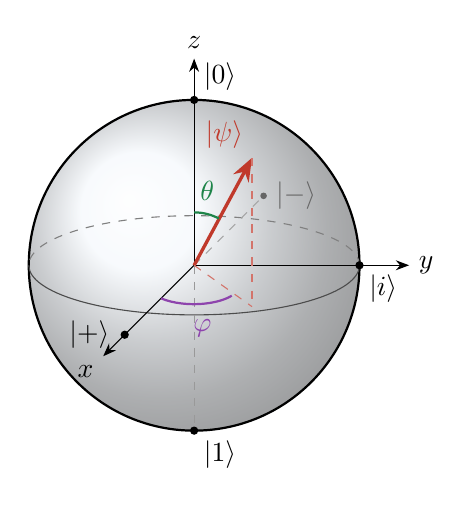
\begin{tikzpicture}[scale=2.1, >=Stealth]
    % sphere
    \shade[ball color=AccentBlue!8, opacity=0.6] (0,0) circle (1);
    \draw[thick] (0,0) circle (1);
    \draw[dashed, black!50] (1,0) arc (0:180:1 and 0.3);
    \draw[black!70] (-1,0) arc (180:360:1 and 0.3);
    % axes
    \draw[->] (0,0) -- (0,1.25) node[above] {$z$};
    \draw[->] (0,0) -- (-0.55,-0.55) node[below left] {$x$};
    \draw[->] (0,0) -- (1.3,0) node[right] {$y$};
    \draw[dashed, black!40] (0,0) -- (0,-1);
    % labels of basis states
    \fill (0,1) circle (0.025) node[above right] {$\ket{0}$};
    \fill (0,-1) circle (0.025) node[below right] {$\ket{1}$};
    \fill (-0.42,-0.42) circle (0.025) node[left=2pt] {$\ket{+}$};
    \draw[dashed, black!35] (0,0) -- (0.42,0.42);
    \fill[black!60] (0.42,0.42) circle (0.02) node[right=1pt, black!60] {$\ket{-}$};
    \fill (1,0) circle (0.025) node[below right] {$\ket{i}$};
    % state vector (front-right, away from the -x direction)
    \coordinate (P) at (0.35,0.65);
    \coordinate (Pp) at (0.35,-0.25);
    \draw[->, very thick, ProbRed] (0,0) -- (P) node[above left=-1pt] {$\ket{\psi}$};
    \draw[dashed, ProbRed!70] (P) -- (Pp);
    \draw[dashed, ProbRed!70] (0,0) -- (Pp);
    % angles
    \draw[OkGreen, thick] (0,0.32) arc (90:62:0.32);
    \node[OkGreen] at (0.08,0.45) {$\theta$};
    \draw[Purple, thick] (-0.2,-0.2) arc (225:325:0.28 and 0.12);
    \node[Purple] at (0.05,-0.38) {$\varphi$};
  \end{tikzpicture}
  \caption{Bloch sphere. Trạng thái $\ket{\psi}$ ở phương trình~\eqref{eq:bloch} ứng với điểm có
  góc cực $\theta$ và góc phương vị $\varphi$.}
  \label{fig:bloch}
\end{figure}

\subsection{Phép đo và collapse}

Như đã nêu ở Mục~\ref{sec:born}, sau phép đo trạng thái \textbf{collapse} (sụp đổ) về đúng ket
tương ứng với bit đo được: kết quả $0$ ứng với $\ket{0}$, kết quả $1$ ứng với $\ket{1}$. Hệ quả thực
tế:
\begin{itemize}[noitemsep]
  \item Một lần đo \textbf{không} cho biết $\alpha, \beta$. Muốn ước lượng phân bố xác suất phải chuẩn
    bị lại trạng thái và đo nhiều lần; mỗi lần gọi là một \textbf{shot}.
  \item Trong Qiskit 2.x, primitive \code{SamplerV2} trả về số lần xuất hiện (\emph{counts}) của mỗi
    chuỗi bit; \code{Statevector} trả về amplitude chính xác nhưng chỉ dùng được với mạch
    \emph{không có} lệnh đo.
\end{itemize}

\subsection{Relative phase và global phase}
\label{sec:phase}

\paragraph{Relative phase.} Hai trạng thái $\ket{+}$ và $\ket{-}$ chỉ khác nhau ở \textbf{dấu của hệ
số đứng trước $\ket{1}$} ($+\tfrac{1}{\sqrt2}$ so với $-\tfrac{1}{\sqrt2}$). Tổng quát, đại lượng phân
biệt chúng là độ lệch pha $\varphi$ giữa $\beta$ và $\alpha$, gọi là \textbf{relative phase} (pha
tương đối); dấu trừ ứng với $\varphi = \pi$, vì $e^{i\pi} = -1$. Tương tự, $\ket{i}$ có
$\varphi = \pi/2$ vì $e^{i\pi/2} = i$. Góc $\varphi$ này chính là góc phương vị trên Bloch sphere ở
phương trình~\eqref{eq:bloch}. Đo trong cơ sở $Z$ không phân biệt được $\ket{+}$ và $\ket{-}$, vì
$|\beta|^2 = \tfrac12$ trong cả hai trường hợp; nhưng đổi cơ sở đo thì được: áp cổng Hadamard trước
khi đo, vì $H\ket{+} = \ket{0}$ và $H\ket{-} = \ket{1}$. Relative phase vì vậy là đại lượng
\textbf{quan sát được}.

\paragraph{Global phase.} \textbf{Global phase} (pha toàn cục) là trường hợp nhân \emph{cả} vector
trạng thái -- tức \emph{mọi} amplitude cùng lúc -- với cùng một hệ số $e^{i\gamma}$:
\begin{equation}
  \ket{\psi'} = e^{i\gamma}\ket{\psi} = e^{i\gamma}\alpha\ket{0} + e^{i\gamma}\beta\ket{1}.
  \label{eq:global}
\end{equation}
Vì mọi amplitude bị quay pha như nhau, độ lệch pha giữa chúng -- relative phase -- không đổi. Hai
lập luận cho thấy global phase \textbf{không thể quan sát được} bằng bất kỳ thí nghiệm nào:
\begin{enumerate}[noitemsep]
  \item \textbf{Mọi phép đo cho cùng phân bố xác suất.} Với phép đo trong một cơ sở trực chuẩn bất kỳ
    $\{\ket{\phi_k}\}$ (không chỉ cơ sở $Z$), quy tắc Born cho
    \[
      P'(k) = \big|\braket{\phi_k|\psi'}\big|^2 = |e^{i\gamma}|^2\,\big|\braket{\phi_k|\psi}\big|^2
      = \big|\braket{\phi_k|\psi}\big|^2 = P(k),
    \]
    vì $|e^{i\gamma}| = 1$.
  \item \textbf{Không cổng nào biến nó thành relative phase.} Với mọi unitary $U$,
    $U\big(e^{i\gamma}\ket{\psi}\big) = e^{i\gamma}\,U\ket{\psi}$: hệ số $e^{i\gamma}$ đi xuyên qua cả
    mạch mà vẫn là hệ số chung, nên đến lúc đo nó vẫn không ảnh hưởng gì (theo lập luận 1).
\end{enumerate}
Vì vậy $\ket{\psi}$ và $e^{i\gamma}\ket{\psi}$ là \textbf{cùng một trạng thái vật lý}. Ví dụ,
$-\ket{-} = \tfrac{1}{\sqrt2}(-\ket{0} + \ket{1})$ chính là $\ket{-}$: cả hai hệ số đều đổi dấu, nên
hệ số trước $\ket{1}$ vẫn ngược dấu với hệ số trước $\ket{0}$. Ngược lại, $\ket{+}$ và $\ket{-}$ là
hai trạng thái khác nhau, vì chỉ \emph{một} hệ số đổi dấu.

Global phase có ba hệ quả được dùng xuyên suốt báo cáo:
\begin{itemize}[noitemsep]
  \item \textbf{Bloch sphere chỉ cần hai góc.} Một qubit có hai amplitude phức (4 tham số thực); trừ
    điều kiện chuẩn hoá và global phase, còn lại đúng 2 tham số. Đây là lý do phương
    trình~\eqref{eq:bloch} được phép chọn hệ số của $\ket{0}$ là số thực không âm $\cos\tfrac{\theta}{2}$.
  \item \textbf{Hai cổng sai khác global phase là cùng một cổng.} Ví dụ $R_X(\pi) = -iX$ và
    $R_Z(\lambda) = e^{-i\lambda/2}P(\lambda)$ (Mục~\ref{sec:gates}). Kết quả mô phỏng có thể khác
    công thức một dấu chung -- như trạng thái Bell $\ket{\Psi^-}$ xuất hiện dưới dạng
    $\tfrac{1}{\sqrt2}(\ket{10}-\ket{01})$ -- mà vẫn đúng. Đây là lý do Qiskit phân biệt
    \code{Operator.equiv} (bỏ qua global phase) với phép so sánh \code{==} (so từng phần tử ma trận).
  \item \textbf{Ngoại lệ quan trọng: cổng controlled.} Global phase của một cổng $U$ không quan sát
    được khi $U$ được áp \emph{vô điều kiện}, nhưng trở thành \emph{relative} phase khi $U$ chỉ được
    áp lúc qubit control bằng 1. Chẳng hạn, áp $-I$ lên target có điều kiện thì chỉ thành phần
    $\ket{1}$ của control bị đổi dấu -- tức tương đương cổng $Z$ trên control. Đây chính là cơ chế
    phase kickback ở Mục~\ref{sec:algorithms}, và là lý do khi tổng hợp cổng controlled, compiler phải
    theo dõi global phase (thuộc tính \code{QuantumCircuit.global\_phase} trong Qiskit) thay vì bỏ nó đi.
\end{itemize}

\begin{keybox}
Relative phase là ``nguyên liệu'' của mọi thuật toán lượng tử: thuật toán ghi thông tin vào phase,
rồi dùng interference (thường là cổng $H$) để biến phase thành xác suất đo được. Global phase thì không
mang thông tin vật lý -- trừ khi nó bị ``gắn điều kiện'' qua một cổng controlled.
\end{keybox}

\subsection{Hệ nhiều qubit và tích tensor}

Hệ gồm hai qubit được mô tả trong không gian $\mathbb{C}^2 \otimes \mathbb{C}^2 = \mathbb{C}^4$.
Hai qubit độc lập ghép lại bằng \textbf{tích tensor} (tích Kronecker):
\begin{equation}
  \ket{a}\otimes\ket{b} =
  \begin{pmatrix}a_0\\a_1\end{pmatrix} \otimes \begin{pmatrix}b_0\\b_1\end{pmatrix}
  = \begin{pmatrix}a_0b_0\\a_0b_1\\a_1b_0\\a_1b_1\end{pmatrix}.
\end{equation}
Tổng quát, $n$ qubit cần $2^n$ amplitude: $\ket{\psi} = \sum_{x \in \{0,1\}^n} c_x \ket{x}$ với
$\sum_x |c_x|^2 = 1$. Không gian trạng thái tăng theo \emph{hàm mũ} -- đây vừa là nguồn sức mạnh của
máy tính lượng tử, vừa là lý do mô phỏng cổ điển nhanh chóng trở nên bất khả thi.

\subsection{Quy ước thứ tự qubit trong Qiskit (little-endian)}
\label{sec:endian}

Khi ghép $n$ qubit bằng tích tensor, phải chọn qubit nào đứng \emph{trái} và qubit nào đứng
\emph{phải} trong ket. Có hai quy ước, và Qiskit dùng quy ước \emph{ngược} với phần lớn giáo trình:
\begin{itemize}[noitemsep]
  \item \textbf{Giáo trình} (Nielsen \& Chuang \cite{nielsen2010}): viết $\ket{q_0 q_1 \dots q_{n-1}}$
    và $\ket{\psi} = \ket{\psi_0}\otimes\ket{\psi_1}\otimes\dots\otimes\ket{\psi_{n-1}}$ -- qubit 0
    đứng \textbf{bên trái}.
  \item \textbf{Qiskit}: viết $\ket{q_{n-1}\dots q_1 q_0}$ và
    $\ket{\psi} = \ket{\psi_{n-1}}\otimes\dots\otimes\ket{\psi_1}\otimes\ket{\psi_0}$ -- qubit 0 đứng
    \textbf{bên phải}.
\end{itemize}

Ở cả hai quy ước, thứ tự viết trong ket luôn trùng với thứ tự các thừa số của tích Kronecker từ trái
sang phải; chỉ có việc qubit nào đứng trái là khác nhau. Nói gọn: \textbf{trong Qiskit, qubit có chỉ
số lớn hơn đứng trước} (bên trái), cả trong ket lẫn trong tích tensor. Nếu ghép theo thứ tự
$\ket{q_0}\otimes\ket{q_1}\otimes\dots$ như giáo trình rồi đưa vào Qiskit, ta được vector bị đảo thứ tự
qubit: với $q_0 = 1, q_1 = 0$, tích $\ket{q_1}\otimes\ket{q_0} = (0,1,0,0)^{\mathsf T}$ là đúng
(chuỗi \code{'01'}), còn $\ket{q_0}\otimes\ket{q_1} = (0,0,1,0)^{\mathsf T}$ lại là trạng thái có
qubit 1 bằng 1.

\paragraph{Vì sao gọi là little-endian.} Mỗi ket cơ sở $\ket{q_{n-1}\dots q_1 q_0}$ ứng với một chỉ số
nguyên $k$ trong vector trạng thái $2^n$ phần tử. Qiskit đọc chuỗi bit đó như cách viết số nhị phân
thông thường, nên
\begin{equation}
  k = \sum_{i=0}^{n-1} q_i\, 2^i = q_0\cdot 2^0 + q_1\cdot 2^1 + \dots + q_{n-1}\cdot 2^{n-1}.
  \label{eq:endian}
\end{equation}
Qubit 0 là \textbf{bit có trọng số thấp nhất} (least significant bit) của chỉ số $k$ -- giống thứ tự
byte ``little-endian'' trong kiến trúc máy tính, nơi phần có trọng số thấp đứng trước. Hệ quả là
qubit 0 xuất hiện ở \textbf{ký tự bên phải cùng} của mọi chuỗi bit mà Qiskit in ra.

\paragraph{Ví dụ.} Mạch 3 qubit, chỉ áp $X$ lên qubit 0:
\begin{itemize}[noitemsep]
  \item Qiskit trả về trạng thái $\ket{001}$, tức chỉ số $k = 1$; vector trạng thái là
    $(0,1,0,0,0,0,0,0)^{\mathsf T}$, và counts là \code{\{'001': ...\}}.
  \item Giáo trình viết cùng trạng thái đó là $\ket{100}$.
\end{itemize}
Hai cách viết mô tả \emph{cùng một} trạng thái vật lý; chỉ có thứ tự ghi các qubit là khác nhau.
Tương tự, áp $H$ lên qubit 0 của mạch 2 qubit cho $\tfrac{1}{\sqrt2}(\ket{00}+\ket{01})$ theo Qiskit
(vector $(1,1,0,0)^{\mathsf T}/\sqrt2$), nhưng là $\tfrac{1}{\sqrt2}(\ket{00}+\ket{10})$ theo giáo trình.

\paragraph{Ảnh hưởng tới ma trận cổng.} Vì thứ tự tensor bị đảo, ma trận của cổng nhiều qubit trong
Qiskit khác ma trận trong giáo trình. Cổng $H$ trên qubit 0 có ma trận $I\otimes H$ (qubit 0 là thừa
số bên phải). Cổng CX với control là qubit 0 và target là qubit 1 (\code{qc.cx(0, 1)}) có ma trận
\[
  \mathrm{CX}^{\text{Qiskit}}_{0\to1} =
  \begin{pmatrix}1&0&0&0\\0&0&0&1\\0&0&1&0\\0&1&0&0\end{pmatrix}
  \qquad\text{thay vì}\qquad
  \mathrm{CX}^{\text{giáo trình}} =
  \begin{pmatrix}1&0&0&0\\0&1&0&0\\0&0&0&1\\0&0&1&0\end{pmatrix}.
\]
Ma trận của Qiskit đổi chỗ $\ket{01}\leftrightarrow\ket{11}$ (các trạng thái có $q_0 = 1$), còn ma
trận giáo trình đổi chỗ $\ket{10}\leftrightarrow\ket{11}$ (các trạng thái có qubit đứng trái bằng 1).
Cả hai đều đúng theo quy ước của mình.

\paragraph{Ảnh hưởng tới kết quả đo.} Chuỗi counts có dạng $c_{n-1}\dots c_1 c_0$: bit cổ điển 0 đứng
bên phải. Ví dụ, đo mạch 3 qubit đã áp $X$ lên qubit 0 và 1 (với \code{measure([0,1,2],[0,1,2])}) cho
chuỗi \code{'011'}. Lưu ý rằng khi \emph{vẽ} mạch, Qiskit lại đặt qubit 0 ở dòng \emph{trên cùng} --
nên thứ tự từ trên xuống trong hình vẽ ngược với thứ tự từ trái sang phải trong chuỗi kết quả.

\paragraph{Cách làm việc an toàn.}
\begin{itemize}[noitemsep]
  \item Khi đọc kết quả, ký tự thứ $i$ \emph{tính từ bên phải} (\code{s[-1-i]} trong Python) là giá trị
    của qubit/bit cổ điển $i$. Muốn đọc theo thứ tự giáo trình thì đảo chuỗi (\code{s[::-1]}).
  \item Khi so sánh với công thức trong giáo trình, dùng \code{QuantumCircuit.reverse\_bits()} (đảo thứ
    tự qubit của mạch) hoặc \code{Statevector.reverse\_qargs()}: mạch ở ví dụ trên sau
    \code{reverse\_bits()} cho đúng \code{'100'}.
  \item Khi ghép trạng thái bằng tích tensor trong Qiskit, phải viết \code{q1.tensor(q0)} (qubit có chỉ
    số lớn đứng trước).
\end{itemize}
Quy ước này xuất hiện ở mọi thuật toán của Mục~\ref{sec:algorithms}: ký tự cuối của chuỗi bí mật $s$
trong Bernstein--Vazirani ứng với qubit 0, và chuỗi kết quả của superdense coding bị đảo so với thứ tự
viết tin nhắn.

\begin{table}[h]
  \centering
  \caption{Tóm tắt các khái niệm cơ bản và cách biểu diễn trong Qiskit.}
  \label{tab:basics}
  \small
  \begin{tabular}{@{}lll@{}}
    \toprule
    \textbf{Khái niệm} & \textbf{Ý nghĩa} & \textbf{Qiskit} \\
    \midrule
    Ket $\ket{0}, \ket{1}$ & computational basis & \code{Statevector.from\_label("0")} \\
    Amplitude $\alpha, \beta$ & số phức, $|\alpha|^2+|\beta|^2=1$ & \code{sv.data}, \code{sv.is\_valid()} \\
    Xác suất & $P(k) = |c_k|^2$ (quy tắc Born) & \code{sv.probabilities\_dict()} \\
    Superposition & tổ hợp tuyến tính các ket & \code{qc.h(0)} \\
    Đo & lấy mẫu + collapse & \code{qc.measure(...)} + \code{SamplerV2} \\
    Relative phase & quan sát được (đổi cơ sở đo) & thêm \code{h} trước \code{measure} \\
    Global phase & không quan sát được & \code{Operator.equiv} \\
    Thứ tự bit & little-endian, qubit 0 bên phải & \code{'001'}: qubit 0 bằng 1 \\
    \bottomrule
  \end{tabular}
\end{table}

%==============================================================
\section{Cổng lượng tử và mạch lượng tử}
\label{sec:gates}
%==============================================================

\subsection{Cổng lượng tử là ma trận unitary}
\label{sec:unitary}

\begin{definition}[Ma trận unitary]
Ma trận vuông phức $U$ gọi là \textbf{unitary} nếu
\begin{equation}
  U^\dagger U = U U^\dagger = I,
  \label{eq:unitary}
\end{equation}
trong đó $U^\dagger = \overline{U}^{\mathsf T}$ là \textbf{liên hợp Hermite} (chuyển vị liên hợp) của
$U$: chuyển vị ma trận rồi lấy liên hợp phức từng phần tử.
\end{definition}

Một cổng lượng tử tác dụng lên $n$ qubit là một ma trận unitary kích thước $2^n \times 2^n$, và áp cổng
lên trạng thái chính là phép nhân ma trận: $\ket{\psi'} = U\ket{\psi}$. Điều kiện~\eqref{eq:unitary}
nói rằng \textbf{nghịch đảo của $U$ chính là $U^\dagger$}, nên luôn tính được trực tiếp. Ví dụ với cổng
Hadamard và cổng phase $S$:
\[
  H^\dagger H = \tfrac12\begin{pmatrix}1&1\\1&-1\end{pmatrix}\begin{pmatrix}1&1\\1&-1\end{pmatrix}
  = \tfrac12\begin{pmatrix}2&0\\0&2\end{pmatrix} = I, \qquad
  S^\dagger S = \begin{pmatrix}1&0\\0&-i\end{pmatrix}\begin{pmatrix}1&0\\0&i\end{pmatrix} = I.
\]
Cổng $S^\dagger$ chính là \code{sdg} trong Qiskit -- tên gọi lấy từ ``S-dagger''.

\paragraph{Vì sao cổng lượng tử bắt buộc phải unitary.} Một cổng phải biến trạng thái hợp lệ thành
trạng thái hợp lệ, tức tổng xác suất luôn bằng 1:
\begin{equation}
  \big\|U\ket{\psi}\big\|^2 = \bra{\psi}U^\dagger U\ket{\psi} = \braket{\psi|\psi} = 1.
\end{equation}
Đẳng thức này đúng với \emph{mọi} $\ket{\psi}$ khi và chỉ khi $U^\dagger U = I$. Vậy tính unitary không
phải một giả thiết tuỳ ý: unitary chính xác là tập các phép biến đổi tuyến tính \textbf{bảo toàn xác
suất}. Về mặt vật lý, một hệ lượng tử cô lập tiến hoá theo phương trình Schrödinger với nghiệm
$U = e^{-i\mathcal{H}t}$, trong đó Hamiltonian $\mathcal{H}$ là một ma trận Hermite; ma trận dạng này
luôn unitary. Thực hiện một cổng trên phần cứng chính là điều khiển Hamiltonian của hệ (bằng xung vi
sóng, laser, \dots) trong một khoảng thời gian xác định.

\begin{table}[h]
  \centering
  \caption{Các tính chất của ma trận unitary và ý nghĩa đối với mạch lượng tử.}
  \label{tab:unitary}
  \small
  \begin{tabularx}{\linewidth}{@{}lX@{}}
    \toprule
    \textbf{Tính chất} & \textbf{Ý nghĩa} \\
    \midrule
    Bảo toàn tích trong: $\braket{U\phi|U\psi} = \braket{\phi|\psi}$ & giữ nguyên ``góc'' giữa các
      trạng thái; hai trạng thái trực giao vẫn trực giao sau cổng \\
    Khả nghịch: $U^{-1} = U^\dagger$ & không cổng nào ``xoá'' thông tin; \code{qc.inverse()} luôn tồn tại \\
    Các cột (và hàng) trực chuẩn & cột thứ $j$ là $U\ket{j}$; ảnh của một cơ sở vẫn là một cơ sở \\
    Trị riêng có môđun 1: $\lambda = e^{i\theta}$ & cổng chỉ ``quay pha'' chứ không co giãn vector \\
    Đóng với phép nhân và tích tensor & ghép cổng nối tiếp ($UV$) hay song song ($U\otimes V$) vẫn được
      unitary, nên cả mạch (không có phép đo) là một unitary \\
    Viết được dưới dạng $U = e^{iA}$, $A$ Hermite & nguồn gốc của các cổng quay
      $R_P(\theta) = e^{-i\theta P/2}$ ở Mục~\ref{sec:1q} \\
    \bottomrule
  \end{tabularx}
\end{table}

\paragraph{So sánh với logic cổ điển.} Cổng AND cổ điển \textbf{không} khả nghịch: đầu ra 0 có thể đến
từ \code{00}, \code{01} hoặc \code{10}, nên thông tin về đầu vào bị mất. Vì vậy AND không thể là một
cổng lượng tử trực tiếp. Muốn tính một hàm cổ điển $f$ trong mạch lượng tử, phải viết lại nó ở dạng
khả nghịch -- cổng Toffoli (một bản AND khả nghịch, Mục~\ref{sec:mq}) hoặc bit-flip oracle
$U_f\ket{x}\ket{y} = \ket{x}\ket{y\oplus f(x)}$ ở Mục~\ref{sec:algorithms}.

\paragraph{Không phải lệnh nào trong mạch cũng unitary.} Phép đo (\code{measure}) và đặt lại qubit
(\code{reset}) làm mất thông tin nên không khả nghịch, và do đó không phải cổng unitary. Đây là lý do
\code{Operator(qc)} và \code{Statevector(qc)} chỉ dùng được với mạch không chứa hai lệnh này. Qiskit
cũng cho phép tạo cổng trực tiếp từ một ma trận bằng \code{UnitaryGate(M)}, và kiểm tra một ma trận
bằng \code{Operator(M).is\_unitary()}.

\paragraph{Số tham số và bài toán synthesis.} Một unitary trên $n$ qubit có $4^n$ tham số thực. Với
một qubit là 4 tham số; bỏ global phase còn 3 -- khớp với ba góc của cổng tổng quát
$U(\theta,\varphi,\lambda)$ ở phương trình~\eqref{eq:u3}. Với hai qubit là 16 tham số, và định lý KAK
cho biết mọi unitary hai qubit cần tối đa 3 cổng CX. Số tham số tăng theo hàm mũ khiến việc phân tích
một unitary tuỳ ý thành chuỗi cổng cơ bản -- bài toán \emph{synthesis} -- trở nên rất khó khi số qubit
tăng (Mục~\ref{sec:synthesis}).

\subsection{Cổng một qubit}
\label{sec:1q}

\paragraph{Nhóm Pauli.}
\begin{equation}
  X = \begin{pmatrix}0&1\\1&0\end{pmatrix}, \qquad
  Y = \begin{pmatrix}0&-i\\i&0\end{pmatrix}, \qquad
  Z = \begin{pmatrix}1&0\\0&-1\end{pmatrix}.
\end{equation}
$X$ là ``NOT lượng tử'' (bit flip, $\ket{0}\leftrightarrow\ket{1}$); $Z$ là phase flip
($\ket{1}\to-\ket{1}$); $Y = iXZ$ làm cả hai. Trên Bloch sphere chúng là các phép quay $180^\circ$
quanh trục tương ứng, và $X^2 = Y^2 = Z^2 = I$.

\paragraph{Hadamard.}
\begin{equation}
  H = \frac{1}{\sqrt2}\begin{pmatrix}1&1\\1&-1\end{pmatrix}, \qquad
  H\ket{0} = \ket{+}, \quad H\ket{1} = \ket{-}, \quad H^2 = I.
\end{equation}
$H$ chuyển qua lại giữa cơ sở $Z$ và cơ sở $X$, nên ``thêm $H$ trước khi đo'' chính là đo trong cơ
sở $X$. Đẳng thức $HZH = X$ (và $HXH = Z$) được dùng liên tục trong thiết kế và tối ưu mạch.

\paragraph{Cổng phase.}
\begin{equation}
  S = \begin{pmatrix}1&0\\0&i\end{pmatrix}, \qquad
  T = \begin{pmatrix}1&0\\0&e^{i\pi/4}\end{pmatrix}, \qquad
  P(\lambda) = \begin{pmatrix}1&0\\0&e^{i\lambda}\end{pmatrix},
  \qquad S^2 = Z,\ T^2 = S.
\end{equation}
Các cổng này chỉ thêm phase cho thành phần $\ket{1}$, tức quay quanh trục $Z$. Vì không đổi
$|\alpha|, |\beta|$ nên đo ngay sau cổng phase không thấy khác biệt gì; phase chỉ lộ ra khi kết hợp
với $H$. Cổng $T$ đặc biệt quan trọng ở Mục~\ref{sec:synthesis}: nó là cổng ``đắt'' nhất trên máy
tính lượng tử chịu lỗi.

\paragraph{Cổng quay.} Với góc tuỳ ý, dùng các cổng rotation
$R_P(\theta) = e^{-i\theta P/2} = \cos\tfrac{\theta}{2}I - i\sin\tfrac{\theta}{2}P$ với
$P \in \{X, Y, Z\}$, ví dụ
\begin{equation}
  R_Y(\theta) = \begin{pmatrix}\cos\frac\theta2 & -\sin\frac\theta2\\[2pt]
                               \sin\frac\theta2 & \cos\frac\theta2\end{pmatrix}, \qquad
  R_Z(\theta) = \begin{pmatrix}e^{-i\theta/2}&0\\0&e^{i\theta/2}\end{pmatrix}.
\end{equation}
Chú ý hệ số $\theta/2$: phải quay $\theta = 2\pi$ mới quay về đúng trạng thái ban đầu kể cả phase.
Ví dụ $R_X(\pi) = -iX$ khác $X$ đúng một global phase.

\paragraph{Cổng tổng quát.} Mọi cổng một qubit đều là trường hợp riêng (sai khác global phase) của
\begin{equation}
  U(\theta,\varphi,\lambda) = \begin{pmatrix}
    \cos\frac\theta2 & -e^{i\lambda}\sin\frac\theta2\\[2pt]
    e^{i\varphi}\sin\frac\theta2 & e^{i(\varphi+\lambda)}\cos\frac\theta2\end{pmatrix}.
  \label{eq:u3}
\end{equation}
Ba tham số thực khớp với ba bậc tự do của $SU(2)$ -- kết quả này là nền tảng của synthesis một qubit
ở Mục~\ref{sec:synthesis}.

\begin{table}[h]
  \centering
  \caption{Tóm tắt các cổng một qubit. Ký hiệu $\mathrm{diag}(a,b)$ là ma trận đường chéo.}
  \label{tab:1q}
  \small
  \begin{tabular}{@{}llll@{}}
    \toprule
    \textbf{Cổng} & \textbf{Qiskit} & \textbf{Quay trên Bloch sphere} & \textbf{Ghi nhớ} \\
    \midrule
    $X$ & \code{qc.x(0)} & $180^\circ$ quanh $X$ & NOT lượng tử \\
    $Y$ & \code{qc.y(0)} & $180^\circ$ quanh $Y$ & bit flip + phase flip \\
    $Z$ & \code{qc.z(0)} & $180^\circ$ quanh $Z$ & phase flip \\
    $H$ & \code{qc.h(0)} & $180^\circ$ quanh $(X+Z)/\sqrt2$ & tạo superposition \\
    $S = \mathrm{diag}(1, i)$ & \code{qc.s(0)} & $90^\circ$ quanh $Z$ & $S^2 = Z$ \\
    $T = \mathrm{diag}(1, e^{i\pi/4})$ & \code{qc.t(0)} & $45^\circ$ quanh $Z$ & $T^2 = S$ \\
    $P(\lambda)$ & \code{qc.p(lam, 0)} & $\lambda$ quanh $Z$ & tổng quát của $Z, S, T$ \\
    $R_X, R_Y, R_Z$ & \code{qc.rx/ry/rz(th, 0)} & $\theta$ quanh trục tương ứng & $R_Y$: $P(1)=\sin^2\frac\theta2$ \\
    \bottomrule
  \end{tabular}
\end{table}

\paragraph{Thứ tự cổng và thứ tự nhân ma trận.} Mạch được vẽ theo thời gian từ trái sang phải, nhưng
ma trận tương ứng được nhân từ phải sang trái. Mạch ``$H$ rồi $X$'' có ma trận $U = X \cdot H$, vì
$X(H\ket{\psi}) = (XH)\ket{\psi}$. Nghịch đảo của cả mạch (\code{qc.inverse()}) đảo ngược thứ tự các
cổng và lấy liên hợp Hermite từng cổng ($T^\dagger$ là \code{tdg}, $S^\dagger$ là \code{sdg}).

\subsection{Cổng nhiều qubit}
\label{sec:mq}

\paragraph{CNOT (CX).} Cổng hai qubit quan trọng nhất: có một qubit \emph{control} và một qubit
\emph{target}; nếu control bằng 1 thì lật target:
\begin{equation}
  \mathrm{CX}\,\ket{c}\ket{t} = \ket{c}\ket{t \oplus c}.
\end{equation}
CX là cổng tạo \emph{tương quan} giữa hai qubit, và cũng là cổng khó thực hiện nhất trên phần cứng.
Vì vậy \textbf{số cổng CX là thước đo chi phí chính} của một mạch -- ý này sẽ xuất hiện lại ở mọi phần
của Mục~\ref{sec:compilation}.

\paragraph{Các cổng khác.} Bảng~\ref{tab:mq} liệt kê các cổng nhiều qubit thường dùng. Một quan hệ
đáng nhớ: kẹp $H$ lên target trước và sau CX thì được CZ, tức $\mathrm{CZ} = (I\otimes H)\,\mathrm{CX}\,(I\otimes H)$
(viết theo thứ tự qubit control $\otimes$ target). Một cổng bất kỳ có thể được biến thành cổng
controlled bằng \code{.to\_gate().control(n)}.

\begin{table}[h]
  \centering
  \caption{Các cổng nhiều qubit thường dùng.}
  \label{tab:mq}
  \small
  \begin{tabular}{@{}lll@{}}
    \toprule
    \textbf{Cổng} & \textbf{Qiskit} & \textbf{Ý nghĩa} \\
    \midrule
    CX / CNOT & \code{qc.cx(c, t)} & control $=1$ thì lật target \\
    CZ & \code{qc.cz(a, b)} & cả hai bằng 1 thì thêm dấu $-$; \textbf{đối xứng} \\
    SWAP & \code{qc.swap(a, b)} & đổi chỗ trạng thái hai qubit; $=3$ CX \\
    Toffoli (CCX) & \code{qc.ccx(c1, c2, t)} & hai control; đủ để làm mọi hàm logic cổ điển khả nghịch \\
    CH, CRX, CP, \dots & \code{qc.ch}, \code{qc.crx}, \code{qc.cp} & bản controlled của cổng một qubit \\
    \bottomrule
  \end{tabular}
\end{table}

\subsection{Entanglement}

\paragraph{Trạng thái Bell.} Chỉ cần hai cổng để tạo ra entanglement:
\begin{equation}
  \ket{00} \xrightarrow{\;H \text{ trên } q_0\;} \tfrac{1}{\sqrt2}\big(\ket{00}+\ket{01}\big)
  \xrightarrow{\;\mathrm{CX}_{0\to1}\;} \tfrac{1}{\sqrt2}\big(\ket{00}+\ket{11}\big) = \ket{\Phi^+}.
\end{equation}

\begin{figure}[h]
  \centering
  \begin{quantikz}
    \lstick{$q_0: \ket{0}$} & \gate{H} & \ctrl{1} & \meter{} \\
    \lstick{$q_1: \ket{0}$} & & \targ{} & \meter{}
  \end{quantikz}
  \caption{Mạch tạo trạng thái Bell $\ket{\Phi^+}$. Kết quả đo chỉ có \code{00} hoặc \code{11},
  mỗi chuỗi xác suất $1/2$.}
  \label{fig:bell}
\end{figure}

Kết quả đo chỉ có \code{00} và \code{11}, không bao giờ có \code{01} hay \code{10}: hai qubit luôn
cho cùng kết quả. Bốn trạng thái Bell
\begin{equation}
  \ket{\Phi^\pm} = \tfrac{1}{\sqrt2}\big(\ket{00}\pm\ket{11}\big), \qquad
  \ket{\Psi^\pm} = \tfrac{1}{\sqrt2}\big(\ket{01}\pm\ket{10}\big)
\end{equation}
trực giao nhau và tạo thành \textbf{Bell basis} của không gian hai qubit. Mở rộng ra $n$ qubit, ta có
trạng thái GHZ $\tfrac{1}{\sqrt2}(\ket{0\dots0}+\ket{1\dots1})$, tạo bằng một cổng $H$ và một chuỗi
CX.

\begin{definition}[Separable và entangled]
Trạng thái hai qubit là \textbf{separable} nếu viết được thành $\ket{\psi_A}\otimes\ket{\psi_B}$;
ngược lại nó là \textbf{entangled}.
\end{definition}

\paragraph{Đo lường entanglement.} Lấy \emph{partial trace} để bỏ qubit $B$, ta được ma trận mật độ
(density matrix) $\rho_A = \Tr_B\ket{\psi}\bra{\psi}$ của qubit $A$. Khi đó:
\begin{itemize}[noitemsep]
  \item \textbf{Purity} $\Tr(\rho_A^2)$ bằng 1 nếu $A$ ở pure state, bằng $0.5$ nếu entangled tối đa.
  \item \textbf{Entropy von Neumann} $S(\rho_A) = -\Tr(\rho_A\log_2\rho_A)$ bằng 0 nếu không
    entangled, bằng 1 nếu entangled tối đa.
\end{itemize}
Với $\ket{\Phi^+}$, giá trị kỳ vọng tính bằng \code{EstimatorV2} cho $\langle ZZ\rangle = +1$ và
$\langle XX\rangle = +1$ (tương quan hoàn hảo trong \emph{cả hai} cơ sở -- điều mà tương quan cổ điển
không làm được), trong khi $\langle ZI\rangle = 0$: riêng từng qubit thì hoàn toàn ngẫu nhiên. Toàn
bộ thông tin nằm ở mối tương quan giữa hai qubit.

\subsection{Tính universal của tập cổng}

Một tập cổng gọi là \textbf{universal} nếu mọi unitary đều biểu diễn được (chính xác hoặc xấp xỉ tuỳ
ý) bằng các cổng trong tập. Hai kết quả kinh điển \cite{nielsen2010, barenco1995}:
\begin{itemize}[noitemsep]
  \item Các cổng một qubit cùng với CX là universal \emph{chính xác}. Đây là cơ sở của các basis
    gates trên phần cứng NISQ, ví dụ $\{\code{rz}, \code{sx}, \code{x}, \code{cx}\}$.
  \item Tập rời rạc Clifford+T $= \{H, S, \mathrm{CX}, T\}$ là universal \emph{xấp xỉ}: mọi unitary
    xấp xỉ được tới sai số $\epsilon$ tuỳ ý. Đây là tập cổng của máy tính lượng tử chịu lỗi.
\end{itemize}
Sự khác biệt giữa hai loại universal này dẫn tới hai bài toán synthesis rất khác nhau ở
Mục~\ref{sec:synthesis}.

\subsection{Quy trình làm việc với Qiskit 2.x}
\label{sec:workflow}

Mọi bài toán trong báo cáo đều đi qua năm bước: (1) \textbf{xây mạch} bằng \code{QuantumCircuit};
(2) \textbf{xem mạch} bằng \code{draw()}, \code{depth()}, \code{count\_ops()}; (3) \textbf{đo} bằng
\code{measure()} hoặc \code{measure\_all()}; (4) \textbf{chạy} bằng một trong ba cách ở
Bảng~\ref{tab:primitives}; (5) \textbf{transpile} về tập cổng và coupling map của thiết bị.

\begin{lstlisting}[caption={Quy trình tối thiểu: tạo trạng thái Bell, transpile và lấy mẫu.}]
from qiskit import QuantumCircuit, transpile
from qiskit_aer import AerSimulator
from qiskit_aer.primitives import SamplerV2

qc = QuantumCircuit(2)
qc.h(0); qc.cx(0, 1)
qc.measure_all()                      # creates a register named "meas"

backend = AerSimulator()
tqc = transpile(qc, backend, optimization_level=2)
res = SamplerV2().run([tqc], shots=1000).result()
print(res[0].data.meas.get_counts())  # ~ {'00': 500, '11': 500}
\end{lstlisting}

\begin{table}[h]
  \centering
  \caption{Ba cách lấy kết quả từ mạch trong Qiskit 2.x.}
  \label{tab:primitives}
  \small
  \begin{tabular}{@{}llll@{}}
    \toprule
    \textbf{Cách} & \textbf{Cho ra} & \textbf{Mạch có \code{measure}?} & \textbf{Dùng khi} \\
    \midrule
    \code{Statevector(qc)} & amplitude chính xác & \textbf{không} được có & học, debug mạch nhỏ \\
    \code{SamplerV2} & counts từ các shot & \textbf{bắt buộc} có & mô phỏng kết quả thật \\
    \code{EstimatorV2} & giá trị kỳ vọng $\langle O\rangle$ & không cần & VQE, đo tương quan \\
    \bottomrule
  \end{tabular}
\end{table}

\begin{warnbox}[Các lỗi hay gặp khi mới dùng Qiskit 2.x]
(1) Đọc nhầm thanh ghi: \code{measure\_all()} tạo thanh ghi \code{meas}, không phải \code{c}.
(2) Gọi \code{Statevector(qc)} khi mạch đã có lệnh đo.
(3) Quên \code{transpile} trước \code{backend.run()}.
(4) Nhầm thứ tự bit: qubit 0 là ký tự bên phải.
(5) So sánh cổng bằng \code{==} trong khi chỉ cần \code{equiv} (khác nhau ở global phase).
Ngoài ra, nhiều tài liệu trên mạng dùng API Qiskit 0.x đã bị gỡ bỏ (\code{execute},
\code{Aer.get\_backend}); API tương ứng hiện nay là các primitive \code{SamplerV2}/\code{EstimatorV2}
và \code{AerSimulator}.
\end{warnbox}

%==============================================================
\section{Các thuật toán lượng tử cơ bản}
\label{sec:algorithms}
%==============================================================

Gần như mọi thuật toán lượng tử cơ bản -- Deutsch--Jozsa, Bernstein--Vazirani, Grover, phase
estimation -- đều dùng chung một thủ thuật:
\begin{quote}
  \emph{Ghi câu trả lời của một hàm vào \textbf{phase} của amplitude, rồi dùng $H$ để biến phase thành
  bit đọc được.}
\end{quote}
Thủ thuật này gọi là \textbf{phase kickback}. Chương này xây dựng nó từ đầu, sau đó áp dụng lần lượt
vào các bài toán với độ tổng quát tăng dần, và kết thúc bằng hai giao thức dùng entanglement làm tài
nguyên chính.

\subsection{Oracle và phase kickback}

\paragraph{Oracle.} Cho hàm $f:\{0,1\}^n\to\{0,1\}$ mà ta chỉ được \emph{gọi} chứ không được xem bên
trong (giống gọi một API). Để đưa $f$ vào mạch lượng tử, nó phải được đóng gói thành một cổng unitary
-- và unitary thì phải khả nghịch. Phép $\ket{x}\mapsto\ket{f(x)}$ nói chung không khả nghịch, nên
cách chuẩn là thêm một qubit phụ (\textbf{ancilla}) và ghi kết quả bằng XOR:
\begin{equation}
  U_f\,\ket{x}\ket{y} = \ket{x}\ket{y\oplus f(x)}.
  \label{eq:oracle}
\end{equation}
Dạng này gọi là \textbf{bit-flip oracle} và luôn khả nghịch ($U_f^2 = I$).

\paragraph{Phase kickback.} Đặt ancilla ở $\ket{-}$ thay vì $\ket{0}$. Vì $\ket{-}$ là vector riêng
của $X$ với trị riêng $-1$, và oracle chính là ``áp $X$ lên ancilla khi $f(x)=1$'', ta có
\begin{equation}
  U_f\,\ket{x}\ket{-} = (-1)^{f(x)}\,\ket{x}\ket{-}.
  \label{eq:kickback}
\end{equation}
Ancilla không đổi; nó chỉ ``đá ngược'' (kick back) dấu $(-1)^{f(x)}$ vào qubit dữ liệu. Câu trả lời
của $f$ đã chuyển từ \emph{bit của ancilla} sang \emph{phase của qubit dữ liệu}. Khi qubit dữ liệu ở
superposition, một lần gọi oracle ghi dấu lên \emph{mọi} giá trị $x$ cùng lúc:
\begin{equation}
  U_f\,\ket{+}\ket{-} = \tfrac{1}{\sqrt2}\Big((-1)^{f(0)}\ket{0} + (-1)^{f(1)}\ket{1}\Big)\ket{-}.
\end{equation}

\subsection{Bài toán Deutsch và Deutsch--Jozsa}

\paragraph{Deutsch.} Cho $f:\{0,1\}\to\{0,1\}$, hỏi $f$ là \emph{hằng} ($f(0)=f(1)$) hay \emph{cân
bằng} ($f(0)\neq f(1)$)? Cổ điển phải gọi $f$ hai lần. Theo phương trình trên, qubit dữ liệu sau
oracle là $\pm\ket{+}$ nếu $f$ hằng và $\pm\ket{-}$ nếu $f$ cân bằng; áp $H$ rồi đo cho đúng
$f(0)\oplus f(1)$ -- chỉ với \textbf{một} lần gọi \cite{deutsch1985}.

\begin{figure}[h]
  \centering
  \begin{quantikz}
    \lstick{$x: \ket{0}$} & \gate{H} & & \gate[2]{U_f} & \gate{H} & \meter{} & \setwiretype{c} \rstick{$f(0)\oplus f(1)$} \\
    \lstick{$\text{anc}: \ket{0}$} & \gate{X} & \gate{H} & & & &
  \end{quantikz}
  \caption{Mạch Deutsch. Ancilla được đưa về $\ket{-}$ bằng $X$ rồi $H$; chỉ đo qubit dữ liệu.}
  \label{fig:deutsch}
\end{figure}

\paragraph{Deutsch--Jozsa.} Mở rộng cho $f:\{0,1\}^n\to\{0,1\}$ với lời hứa $f$ hoặc hằng, hoặc cân
bằng (đúng một nửa đầu vào cho 0) \cite{deutsch1992}. Cổ điển, trong trường hợp xấu nhất cần
$2^{n-1}+1$ lần gọi để chắc chắn. Mạch lượng tử giống hệt Deutsch với $n$ qubit dữ liệu:
$H^{\otimes n}$ -- oracle -- $H^{\otimes n}$ -- đo. Kết quả \textbf{toàn 0} nghĩa là $f$ hằng, bất
kỳ kết quả nào khác nghĩa là $f$ cân bằng. Lý do: amplitude của $\ket{0^n}$ sau cùng là
$\frac{1}{2^n}\sum_x(-1)^{f(x)}$, bằng $\pm1$ nếu $f$ hằng và bằng $0$ nếu $f$ cân bằng.

\begin{warnbox}
Chỉ đo qubit dữ liệu. Nếu dùng \code{measure\_all()}, ancilla (đang ở $\ket{-}$) cũng bị đo và cho bit
ngẫu nhiên, làm chuỗi counts có một bit ``rác'' khiến ta tưởng thuật toán sai.
\end{warnbox}

\subsection{Bernstein--Vazirani}

\paragraph{Bài toán.} Có chuỗi bí mật $s\in\{0,1\}^n$; oracle tính
$f(x) = s\cdot x \bmod 2 = s_0x_0\oplus\dots\oplus s_{n-1}x_{n-1}$. Tìm $s$ \cite{bernstein1997}.

Cổ điển, mỗi lần gọi (với $x$ là một vector đơn vị) chỉ lấy được \textbf{một} bit của $s$, nên cần
$n$ lần. Lượng tử dùng đúng mạch Deutsch--Jozsa. Oracle được hiện thực bằng một cổng CX từ qubit $i$
vào ancilla cho mỗi $i$ có $s_i=1$. Sau oracle, phase kickback cho trạng thái
\begin{equation}
  \frac{1}{\sqrt{2^n}}\sum_{x}(-1)^{s\cdot x}\ket{x} = H^{\otimes n}\ket{s}.
\end{equation}
Vì $H^{\otimes n}$ là nghịch đảo của chính nó, lớp $H^{\otimes n}$ cuối cùng đưa trạng thái về đúng
$\ket{s}$: đo ra $s$ với xác suất \textbf{100\%}, chỉ sau \textbf{một} lần gọi. Đây là ví dụ gọn nhất
về \emph{interference có chủ đích}: các amplitude sai triệt tiêu nhau, amplitude đúng cộng dồn lại.

\begin{keybox}[Lợi thế ở đây đo bằng gì?]
Thước đo là \textbf{số lần gọi oracle} (query complexity), không phải tổng số cổng: bên trong oracle
BV vẫn có tới $n$ cổng CX. Deutsch--Jozsa và BV là các bài toán được \emph{thiết kế} để lợi thế lộ ra;
chúng không nói lên rằng máy lượng tử nhanh hơn trong các bài toán thực tế.
\end{keybox}

\subsection{Thuật toán Grover}

Khác với hai bài toán trên, Grover giải một bài toán \textbf{hoàn toàn tổng quát}: tìm kiếm không cấu
trúc \cite{grover1996}. Có $N = 2^n$ khả năng, trong đó $M$ khả năng là ``nghiệm''; ta chỉ có oracle
trả lời ``đây có phải nghiệm không''. Cổ điển cần trung bình $N/2$ lần thử; Grover cần khoảng
$\frac{\pi}{4}\sqrt{N/M}$ lần -- lợi thế \textbf{bình phương}.

\paragraph{Phase oracle.} Đánh dấu nghiệm bằng dấu âm:
$U_\omega\ket{x} = -\ket{x}$ nếu $x=\omega$, ngược lại giữ nguyên. Hiện thực: áp $X$ lên các qubit
bằng 0 trong $\omega$, áp một cổng multi-controlled $Z$, rồi áp $X$ trả lại.

\paragraph{Diffuser.} Dấu âm một mình không đổi xác suất ($|-a|^2 = |a|^2$). Bước \textbf{diffuser}
$D = H^{\otimes n}(2\ket{0}\bra{0}-I)H^{\otimes n}$ thực hiện phép \emph{lật quanh giá trị trung
bình} (inversion about the mean): $a_k \mapsto 2\bar a - a_k$. Amplitude âm nằm dưới trung bình rất xa
nên sau khi lật nhảy lên trên trung bình -- tức được khuếch đại.

\begin{figure}[h]
  \centering
  \begin{quantikz}[row sep=0.25cm]
    \lstick[3]{$\ket{0}^{\otimes n}$} & \gate{H} & \gate[3]{U_\omega}\gategroup[3,steps=4,style={dashed,rounded corners,fill=AccentBlue!8,inner xsep=2pt},background,label style={label position=above,anchor=south,yshift=-0.1cm}]{lặp $k \approx \frac{\pi}{4}\sqrt{N/M}$ lần: oracle + diffuser} & \gate{H} & \gate[3]{2\ket{0}\bra{0}-I} & \gate{H} & \meter{} \\
    & \gate{H} & & \gate{H} & & \gate{H} & \meter{} \\
    & \gate{H} & & \gate{H} & & \gate{H} & \meter{}
  \end{quantikz}
  \caption{Cấu trúc thuật toán Grover: khởi tạo superposition đều, rồi lặp $k$ vòng gồm oracle
  $U_\omega$ và diffuser.}
  \label{fig:grover}
\end{figure}

\paragraph{Phân tích hình học.} Trạng thái luôn nằm trong mặt phẳng hai chiều sinh bởi ``tổng các
nghiệm'' và ``tổng các phi nghiệm''. Mỗi vòng Grover (oracle + diffuser) là một phép \emph{quay} góc
$2\theta$ về phía nghiệm, với $\sin\theta = \sqrt{M/N}$. Sau $k$ vòng,
\begin{equation}
  P(k) = \sin^2\big((2k+1)\theta\big), \qquad
  k_{\text{opt}} \approx \frac{\pi}{4}\sqrt{\frac{N}{M}}.
  \label{eq:grover}
\end{equation}
Công thức~\eqref{eq:grover} nói hai điều: số vòng tối ưu tăng như $O(\sqrt N)$, và \textbf{lặp nhiều
hơn không tốt hơn} -- quá $k_{\text{opt}}$, trạng thái quay vượt qua nghiệm và xác suất giảm
(Hình~\ref{fig:grover-prob}). Với $n=3$, $M=1$: $k_{\text{opt}}=2$ và $P\approx 94.5\%$, khớp với
kết quả mô phỏng trong notebook.

\begin{figure}[h]
  \centering
  \begin{tikzpicture}
    \begin{axis}[
      width=0.78\linewidth, height=5.2cm,
      xlabel={Số vòng Grover $k$}, ylabel={$P(k)$},
      xmin=-0.5, xmax=12.5, ymin=0, ymax=1.08,
      xtick={0,1,...,12}, ytick={0,0.25,0.5,0.75,1},
      grid=major, grid style={black!10},
      legend style={at={(0.5,1.03)}, anchor=south, legend columns=2, font=\footnotesize},
    ]
      \addplot[ybar, bar width=7pt, fill=AccentBlue!60, draw=AccentBlue,
               samples at={0,1,...,12}]
        {sin((2*x+1)*asin(0.25))^2};
      \addlegendentry{$N=16,\ M=1$}
      \addplot[only marks, mark=*, ProbRed, samples at={0,1,...,12}]
        {sin((2*x+1)*asin(sqrt(4/16)))^2};
      \addlegendentry{$N=16,\ M=4$}
      \draw[dashed, OkGreen, thick] (axis cs:3,0) -- (axis cs:3,1.05);
      \node[OkGreen, font=\footnotesize, anchor=west, fill=white, inner sep=1pt] at (axis cs:3.15,0.12) {$k_{\text{opt}}=3$};
    \end{axis}
  \end{tikzpicture}
  \caption{Xác suất tìm được nghiệm theo số vòng Grover (phương trình~\eqref{eq:grover}). Với một
  nghiệm trong 16 phần tử, xác suất đạt cực đại $96\%$ tại $k=3$ rồi giảm; với 4 nghiệm, số vòng
  tối ưu chỉ là 1.}
  \label{fig:grover-prob}
\end{figure}

\subsection{No-cloning, teleportation và superdense coding}

\paragraph{Định lý no-cloning.} Không tồn tại unitary nào sao chép được một trạng thái tuỳ ý:
$\ket{\psi}\ket{0}\mapsto\ket{\psi}\ket{\psi}$ với mọi $\psi$ \cite{wootters1982}. Chứng minh ngắn
dựa vào tính tuyến tính: nếu một mạch sao chép được $\ket{0}$ và $\ket{1}$ (CX làm được điều này),
thì tác dụng của nó lên $\ket{+}$ buộc phải là $\frac{1}{\sqrt2}(\ket{00}+\ket{11})$ -- một trạng thái
Bell -- chứ không phải $\ket{+}\ket{+}$.

\paragraph{Teleportation.} Alice muốn chuyển trạng thái chưa biết $\ket{\psi}$ của qubit $q_0$ cho Bob
\cite{bennett1993teleport}. Hai người chia sẵn một cặp Bell ($q_1$ của Alice, $q_2$ của Bob). Alice
áp CX$(q_0,q_1)$ rồi $H(q_0)$, đo hai qubit của mình được hai bit $m_0, m_1$, gửi chúng cho Bob qua
kênh cổ điển; Bob áp $X^{m_1}$ rồi $Z^{m_0}$ và thu được đúng $\ket{\psi}$. Bước sửa cuối dùng
\textbf{mid-circuit measurement} và điều khiển cổ điển (trong Qiskit 2.x: \code{with qc.if\_test(...)}).

\begin{figure}[h]
  \centering
  \begin{quantikz}[row sep=0.3cm]
    \lstick{$q_0: \ket{\psi}$} & & & \ctrl{1} & \gate{H} & \meter{} & \setwiretype{c} \rstick{$m_0$} \\
    \lstick{$q_1: \ket{0}$} & \gate{H} & \ctrl{1} & \targ{} & & \meter{} & \setwiretype{c} \rstick{$m_1$} \\
    \lstick{$q_2: \ket{0}$} & & \targ{} & & & & \gate{X^{m_1}} & \gate{Z^{m_0}} & \rstick{$\ket{\psi}$}
  \end{quantikz}
  \caption{Giao thức teleportation. Hai cổng đầu tạo cặp Bell giữa Alice ($q_1$) và Bob ($q_2$).
  Hai cổng sửa của Bob được điều khiển bởi hai bit cổ điển $m_0, m_1$.}
  \label{fig:teleport}
\end{figure}

Teleportation không vi phạm thuyết tương đối: trước khi nhận hai bit cổ điển, qubit của Bob ở trạng
thái hoàn toàn ngẫu nhiên (đo cho 50/50). Nó cũng không vi phạm no-cloning: trạng thái gốc của Alice
bị phá huỷ khi đo. Do mạch có phép đo giữa chừng, không thể kiểm tra bằng \code{Statevector}; cách
kiểm tra chuẩn là áp nghịch đảo của mạch chuẩn bị $\ket{\psi}$ lên qubit của Bob rồi đo -- phải được
\code{0} trong 100\% số shot.

\paragraph{Superdense coding.} Chiều ngược lại: gửi \textbf{2 bit cổ điển} bằng \textbf{1 qubit}
\cite{bennett1992dense}. Với một cặp Bell chia trước, Alice áp $I$, $X$, $Z$ hoặc $ZX$ lên qubit của
mình tuỳ theo hai bit cần gửi; bốn phép này biến cặp Bell thành bốn trạng thái Bell trực giao, nên Bob
phân biệt chắc chắn bằng cách đảo mạch tạo Bell (CX rồi $H$) và đo. Tổng số qubit được truyền vẫn là
2 (một qubit đi trước khi chia cặp), nên không vi phạm giới hạn Holevo.

\subsection{Tổng kết chương}

\begin{table}[h]
  \centering
  \caption{So sánh các thuật toán và giao thức đã trình bày.}
  \label{tab:algo-summary}
  \small
  \begin{tabularx}{\linewidth}{@{}lllX@{}}
    \toprule
    \textbf{Bài toán} & \textbf{Cổ điển} & \textbf{Lượng tử} & \textbf{Cơ chế chính} \\
    \midrule
    Deutsch & 2 lần gọi & 1 lần gọi & phase kickback + $H$ \\
    Deutsch--Jozsa & $2^{n-1}+1$ lần gọi & 1 lần gọi & phase kickback + $H^{\otimes n}$ \\
    Bernstein--Vazirani & $n$ lần gọi & 1 lần gọi & interference về đúng $\ket{s}$ \\
    Grover & $O(N)$ & $O(\sqrt{N})$ & oracle + diffuser (khuếch đại amplitude) \\
    Teleportation & -- & 1 qubit $=$ 1 cặp Bell + 2 bit & entanglement + điều khiển cổ điển \\
    Superdense coding & -- & 2 bit $=$ 1 cặp Bell + 1 qubit & 4 trạng thái Bell trực giao \\
    \bottomrule
  \end{tabularx}
\end{table}

Điểm chung về bản chất: các thuật toán này \textbf{không} tính $f$ nhanh hơn. Chúng trả lời một câu
hỏi \emph{toàn cục} về $f$ mà không cần biết từng giá trị $f(x)$, nhờ ghi thông tin vào phase và
dùng interference để đọc ra. Tất cả đều được viết dưới dạng mạch lý tưởng -- dùng cổng
multi-controlled, CX giữa hai qubit bất kỳ. Chương tiếp theo xem điều gì xảy ra khi đưa các mạch đó
lên phần cứng thật.

%==============================================================
\section{Biên dịch mạch lượng tử}
\label{sec:compilation}
%==============================================================

Các chương trước coi mạch lượng tử là một đối tượng toán học: viết \code{qc.ccx(0,1,2)} thì có cổng
Toffoli, viết \code{qc.cx(0,4)} thì có CX giữa qubit 0 và 4. Phần cứng thật không cho phép điều đó.
Chương này phân tích quá trình \textbf{compilation} -- dịch mạch lý tưởng thành mạch mà một thiết bị
cụ thể chạy được, với sai số nhỏ nhất có thể -- và nhìn nó như một \textbf{bài toán tối ưu}.

\subsection{Phát biểu bài toán}

\begin{definition}[Quantum circuit compilation]
Cho mạch $C$ trên $n$ qubit logic, và một thiết bị mô tả bởi bộ ba
$\mathcal{T} = (\mathcal{G}, G_{\text{cm}}, \varepsilon)$, trong đó $\mathcal{G}$ là tập
\textbf{basis gates}, $G_{\text{cm}} = (V, E)$ là \textbf{coupling map} (đỉnh là qubit vật lý, cạnh
là cặp qubit cho phép cổng hai qubit) và $\varepsilon$ gán sai số cho từng cổng trên từng qubit/cạnh.
Tìm mạch $C'$ sao cho: (i) $C'$ chỉ dùng cổng trong $\mathcal{G}$; (ii) mọi cổng hai qubit của $C'$
nằm trên một cạnh của $G_{\text{cm}}$; (iii) $C'$ tương đương với $C$ (cùng unitary, sai khác một
hoán vị qubit đã biết và global phase); và (iv) $C'$ tối ưu theo một hàm cost (Mục~\ref{sec:cost}).
\end{definition}

Trong Qiskit, bộ ba $\mathcal{T}$ được đóng gói thành đối tượng \code{Target}. Điều kiện (iii) là chỗ
dễ sai nhất khi tự viết compiler, và Mục~\ref{sec:verify} sẽ chỉ ra vì sao.

\subsection{Pipeline của transpiler}

Qiskit không biên dịch bằng một hàm lớn duy nhất mà chạy một chuỗi \textbf{pass}, mỗi pass làm một
việc nhỏ. Các pass được nhóm thành sáu \textbf{stage} cố định (Hình~\ref{fig:pipeline},
Bảng~\ref{tab:stages}); hàm \code{generate\_preset\_pass\_manager} dựng sẵn chuỗi này theo tham số
\code{optimization\_level} và trả về một \code{StagedPassManager}.

\begin{figure}[h]
  \centering
  \begin{tikzpicture}[node distance=0.35cm, every node/.style={font=\small}]
    \node[box=black, minimum width=1.7cm] (in) {\code{QuantumCircuit}};
    \node[box=AccentBlue, right=of in, minimum width=1.2cm] (init) {\code{init}};
    \node[box=OkGreen, right=of init, minimum width=1.2cm] (lay) {\code{layout}};
    \node[box=OkGreen, right=of lay, minimum width=1.2cm] (rou) {\code{routing}};
    \node[box=OrangeYellow, right=of rou, minimum width=1.2cm] (tra) {\code{translation}};
    \node[box=Purple, right=of tra, minimum width=1.2cm] (opt) {\code{optimization}};
    \node[box=AccentBlue, below=0.9cm of opt, minimum width=1.2cm] (sch) {\code{scheduling}};
    \node[box=ProbRed, left=of sch, minimum width=1.7cm] (out) {mạch chạy được};
    \draw[arr] (in) -- (init);
    \draw[arr] (init) -- (lay);
    \draw[arr] (lay) -- (rou);
    \draw[arr] (rou) -- (tra);
    \draw[arr] (tra) -- (opt);
    \draw[arr] (opt) -- (sch);
    \draw[arr] (sch) -- (out);
    \draw[arr, dashed] (opt.north east) to[out=70, in=110, looseness=1.6] node[above, font=\footnotesize] {lặp tới khi hội tụ} (opt.north west);
    \node[draw=black!25, dashed, rounded corners, fit=(lay)(rou), inner sep=4pt,
          label={[font=\footnotesize, text=OkGreen]below:connectivity}] {};
  \end{tikzpicture}
  \caption{Sáu stage của pass manager trong Qiskit. Layout và routing giải quyết ràng buộc
  connectivity; translation giải quyết ràng buộc basis gates; optimization lặp đến khi không giảm
  được nữa.}
  \label{fig:pipeline}
\end{figure}

\begin{table}[h]
  \centering
  \caption{Sáu stage của \code{StagedPassManager} và các pass tiêu biểu.}
  \label{tab:stages}
  \small
  \begin{tabularx}{\linewidth}{@{}lXl@{}}
    \toprule
    \textbf{Stage} & \textbf{Nhiệm vụ} & \textbf{Pass tiêu biểu} \\
    \midrule
    \code{init} & chuẩn hoá đầu vào, phân rã cổng $\ge 3$ qubit & \code{HighLevelSynthesis},\\ & & \code{UnitarySynthesis} \\
    \code{layout} & chọn qubit vật lý cho từng qubit logic & \code{SabreLayout}, \code{VF2Layout} \\
    \code{routing} & chèn SWAP để mọi cổng hai qubit hợp lệ & \code{SabreSwap}, \code{BasicSwap} \\
    \code{translation} & dịch mọi cổng về basis gates & \code{BasisTranslator} \\
    \code{optimization} & huỷ, gộp cổng; lặp tới khi hội tụ & \code{Optimize1qGatesDecomposition},\\ & & \code{CommutativeCancellation} \\
    \code{scheduling} & gán thời điểm thực thi, chèn delay & \code{ALAPScheduleAnalysis}, \code{PadDelay} \\
    \bottomrule
  \end{tabularx}
\end{table}

Theo dõi từng pass bằng tham số \code{callback} của \code{pm.run} cho thấy, với mạch ví dụ ở
Hình~\ref{fig:motivation}, \textbf{47 pass} được chạy ở \code{optimization\_level=2}.
\code{BasisTranslator} là pass làm mạch \emph{nở ra} nhiều nhất (dịch \code{ccx}, \code{ry},
\code{cz} ra basis), các pass optimization sau đó \emph{co} mạch lại, còn phần lớn pass không đổi
mạch -- chúng là pass phân tích. Có hai loại pass:
\begin{itemize}[noitemsep]
  \item \code{AnalysisPass}: đọc mạch, ghi kết quả vào \code{property\_set} -- một từ điển dùng
    chung cho cả pipeline và là kênh duy nhất để các pass trao đổi thông tin; \textbf{không} sửa mạch.
  \item \code{TransformationPass}: nhận mạch, trả về mạch mới.
\end{itemize}

\subsection{\code{DAGCircuit} và front layer}

\code{QuantumCircuit} là một \emph{danh sách} cổng theo thứ tự viết. Thứ tự đó giả tạo: hai cổng trên
hai qubit khác nhau viết trước--sau nhưng thực ra độc lập. Vì vậy pass làm việc trên biểu diễn trung
gian \code{DAGCircuit} -- một \textbf{đồ thị có hướng không chu trình} (directed acyclic graph) mà
đỉnh là cổng và cạnh là qubit/clbit nối hai cổng liên tiếp. Cạnh biểu diễn quan hệ phụ thuộc thật:
cổng $B$ nằm sau cổng $A$ trên DAG nghĩa là $B$ \emph{phải} chờ $A$.

\begin{definition}[Front layer]
\textbf{Front layer} $F$ của một DAG là tập các cổng không còn cổng nào chưa thực thi đứng trước nó
-- tức tập cổng \emph{có thể thực thi ngay}.
\end{definition}

Front layer là khái niệm trung tâm của routing (Mục~\ref{sec:routing}) và chính là thành phần chính
của \emph{state} khi phát biểu routing thành bài toán MDP (Mục~\ref{sec:mdp}).

\subsection{Hàm cost: thế nào là một mạch ``tốt''?}
\label{sec:cost}

Có bốn thước đo hay dùng, và chúng \textbf{không cùng chiều}:
\begin{itemize}[noitemsep]
  \item \textbf{depth} -- số lớp cổng trên đường dài nhất; tỉ lệ với thời gian chạy, cần so với thời
    gian decoherence $T_2$.
  \item \textbf{size} -- tổng số cổng.
  \item \textbf{số cổng hai qubit} -- chi phối sai số, nên có trọng số lớn nhất.
  \item \textbf{số SWAP} -- giá phải trả cho connectivity; mỗi SWAP bằng 3 CX.
\end{itemize}
Một ước lượng thô nhưng hữu dụng: nếu mạch có $m$ cổng hai qubit, mỗi cổng lỗi với xác suất
$\epsilon$, thì xác suất chạy trọn mạch không lỗi là
\begin{equation}
  P_{\text{thành công}} \approx (1-\epsilon)^m \approx e^{-\epsilon m}, \qquad
  \text{hoặc chính xác hơn}\quad P_{\text{thành công}} \approx \prod_{g} (1 - \epsilon_g),
  \label{eq:psuccess}
\end{equation}
trong đó tích lấy trên mọi cổng $g$ với sai số $\epsilon_g$ riêng của qubit/cạnh mà nó chạy trên
đó (đọc từ \code{Target}). Bảng~\ref{tab:optlevel} cho thấy tác động của compiler: cùng mạch, cùng
thiết bị giả lập (\code{GenericBackendV2}, sai số \cx{} trung bình $3.1\times10^{-3}$), chỉ đổi
\code{optimization\_level} đã nâng xác suất thành công từ $0.89$ lên $0.94$.

\begin{table}[h]
  \centering
  \caption{Ảnh hưởng của \code{optimization\_level} lên mạch ví dụ (5 qubit, coupling map
  \code{line(5)}). $P$ tính theo~\eqref{eq:psuccess} chỉ với các cổng \cx{}.}
  \label{tab:optlevel}
  \small
  \begin{tabular}{@{}cccccc@{}}
    \toprule
    \code{optimization\_level} & depth & size & số \cx{} & cổng 1 qubit & $P_{\text{thành công}}$ \\
    \midrule
    0 & 57 & 82 & 37 & 40 & 0.892 \\
    1 & 46 & 67 & 31 & 31 & 0.908 \\
    2 & 40 & 65 & \textbf{19} & 41 & \textbf{0.943} \\
    3 & 40 & 65 & 19 & 41 & 0.943 \\
    \bottomrule
  \end{tabular}
\end{table}

Ba bài toán con quan trọng nhất của compiler -- \emph{layout}, \emph{routing} và \emph{synthesis} --
được trình bày lần lượt dưới đây.

%--------------------------------------------------------------
\subsection{Layout: gán qubit logic cho qubit vật lý}
\label{sec:layout}

Mạch dùng các \textbf{qubit logic} $q_0, q_1, \dots$ -- chỉ là nhãn. Thiết bị có các \textbf{qubit
vật lý} $Q_0, Q_1, \dots$ nối với nhau theo coupling map. \textbf{Layout} (còn gọi là
\emph{initial mapping} hay \emph{qubit allocation}) là một đơn ánh
$\pi: \{q_i\} \to \{Q_j\}$.

\paragraph{Coupling map và distance matrix.} Bậc trung bình của coupling map đo độ ``chật'' của
thiết bị: \code{line(5)} có bậc 1.6, \code{ring(5)} 2.0, \code{grid(2,4)} 2.5, \code{full(5)} 4.0;
kiến trúc heavy-hex của IBM chỉ khoảng 2.1. Dữ liệu quan trọng nhất của coupling map là
\textbf{distance matrix} $D$, với $D[i][j]$ là độ dài đường đi ngắn nhất giữa $Q_i$ và $Q_j$; cổng
hai qubit giữa $Q_i$ và $Q_j$ cần ít nhất $D[i][j]-1$ SWAP. Mọi heuristic routing đều tính cost từ $D$.

\paragraph{Layout là bài toán subgraph isomorphism.} Mỗi mạch có một \textbf{interaction graph}:
đỉnh là qubit logic, cạnh là cặp qubit có ít nhất một cổng hai qubit. Nếu interaction graph
\emph{nhúng được} vào coupling map, tồn tại layout cần \textbf{0 SWAP}. Tìm phép nhúng đó là bài toán
\emph{subgraph isomorphism} -- NP-đầy đủ; khi không nhúng được, tối thiểu hoá số SWAP cũng là
NP-hard \cite{siraichi2018allocation}.

\begin{table}[h]
  \centering
  \caption{Bốn layout pass của Qiskit, và kết quả trên cùng một mạch 4 qubit có 3 cổng \cx{}
  trên coupling map \code{line(4)}.}
  \label{tab:layout}
  \small
  \begin{tabular}{@{}llcc@{}}
    \toprule
    \textbf{Pass} & \textbf{Cách làm} & \textbf{SWAP} & \textbf{depth} \\
    \midrule
    \code{TrivialLayout} & $q_i \to Q_i$, làm baseline & 3 & 5 \\
    \code{DenseLayout} & chọn vùng con dày nhất của thiết bị, không nhìn mạch & 3 & 5 \\
    \code{VF2Layout} & subgraph isomorphism chính xác (VF2++ \cite{juttner2018vf2pp}) & \textbf{0} & \textbf{3} \\
    \code{SabreLayout} & heuristic SABRE, làm layout \emph{và} routing nhiều lần thử & -- & -- \\
    \bottomrule
  \end{tabular}
\end{table}

Bảng~\ref{tab:layout} cho thấy giá trị của layout: cùng một mạch, chỉ khác nhau ở cách đánh số qubit,
mà một bên cần 3 SWAP (tức 9 cổng \cx{} thêm vào một mạch vốn chỉ có 3 cổng \cx{}), bên kia cần 0.

\paragraph{Noise-aware layout.} Các cạnh của coupling map không như nhau: trên thiết bị giả lập, cạnh
tệ nhất có sai số gấp 4.1 lần cạnh tốt nhất. Pass \code{VF2PostLayout} tìm một phép nhúng khác cùng
hình dạng nhưng trên các cạnh tốt hơn. Trong thí nghiệm, nó giảm tổng sai số của một mạch 3 cổng
\cx{} khoảng \textbf{56\%} (xác suất không lỗi từ $0.9884$ lên $0.9949$) mà \emph{không bớt cổng nào}.

%--------------------------------------------------------------
\subsection{Routing: chèn SWAP}
\label{sec:routing}

Với mạch thực tế, interaction graph luôn dày hơn coupling map nên không layout nào đủ tốt; compiler
buộc phải chèn SWAP để đưa các cặp qubit cần tương tác lại cạnh nhau. Mọi router -- từ
\code{BasicSwap}, tới SABRE, tới một RL policy -- đều là cùng một vòng lặp (Thuật toán~\ref{alg:routing}),
chỉ khác nhau ở \textbf{một dòng}: chọn SWAP nào.

\begin{algorithm}[h]
  \caption{Vòng lặp routing tổng quát}
  \label{alg:routing}
  \begin{algorithmic}[1]
    \Require DAG của mạch, coupling map $G_{\text{cm}}=(V,E)$, layout ban đầu $\pi$
    \Ensure mạch hợp lệ với $G_{\text{cm}}$ và layout cuối $\pi$
    \State $F \gets$ front layer của DAG
    \While{DAG còn cổng}
      \State $\mathcal{E} \gets \{g \in F : g$ một qubit, hoặc $(\pi(g_1),\pi(g_2)) \in E\}$
      \If{$\mathcal{E} \neq \emptyset$}
        \State thực thi mọi cổng trong $\mathcal{E}$, xoá khỏi DAG, cập nhật $F$
      \Else
        \State chọn cạnh $(a,b) \in E$ \Comment{\textcolor{ProbRed}{quyết định duy nhất}}
        \State chèn $\mathrm{SWAP}(a,b)$, cập nhật $\pi$
      \EndIf
    \EndWhile
  \end{algorithmic}
\end{algorithm}

Tối thiểu hoá số SWAP là NP-hard, nên mọi router thực tế dùng heuristic. Thuật toán \textbf{SABRE}
\cite{li2019sabre} -- router mặc định của Qiskit (\code{SabreSwap}) -- chọn SWAP làm giảm nhiều nhất
một hàm cost $H$ tính trên distance matrix. Gọi $F$ là front layer và $E_{\text{ext}}$ là
\emph{extended set} (vài lớp cổng hai qubit kế tiếp), SABRE có ba heuristic:
\begin{align}
  H_{\text{basic}} &= \frac{1}{|F|}\sum_{g\in F} D\big[\pi(g_1)\big]\big[\pi(g_2)\big], \label{eq:hbasic}\\
  H_{\text{lookahead}} &= H_{\text{basic}} + W\cdot\frac{1}{|E_{\text{ext}}|}\sum_{g\in E_{\text{ext}}} D\big[\pi(g_1)\big]\big[\pi(g_2)\big], \label{eq:hlook}\\
  H_{\text{decay}} &= \max\big(\mathrm{decay}[a], \mathrm{decay}[b]\big)\cdot H_{\text{lookahead}}, \label{eq:hdecay}
\end{align}
trong đó $(a,b)$ là cạnh ứng viên và $\mathrm{decay}[\cdot]$ tăng mỗi khi một qubit vừa bị SWAP, để
tránh dồn mọi SWAP vào cùng một qubit làm depth tăng vọt. \code{decay} là mặc định, và đây là hàm
mục tiêu mà một RL policy cần vượt qua -- lưu ý nó đã cân bằng giữa số SWAP và depth chứ không chỉ
đếm SWAP. Ngoài ra, \code{SabreLayout} chạy routing \emph{xuôi rồi ngược} nhiều lần để tinh chỉnh
layout ban đầu, nên layout và routing trong SABRE không tách rời.

\begin{table}[h]
  \centering
  \caption{So sánh các router trên một mạch 5 qubit (29 \cx{}, depth 71), coupling map
  \code{line(5)}, layout tầm thường. \code{mini\_router} là router tự cài đặt theo đúng công
  thức~\eqref{eq:hbasic}.}
  \label{tab:routers}
  \small
  \begin{tabular}{@{}lcc@{}}
    \toprule
    \textbf{Router} & \textbf{SWAP} & \textbf{depth} \\
    \midrule
    \code{BasicSwap} (đường ngắn nhất, không nhìn trước) & 14 & 123 \\
    \code{LookaheadSwap} & 7 & 89 \\
    \code{SabreSwap} -- \code{basic} & 8 & 118 \\
    \code{SabreSwap} -- \code{lookahead} & 8 & 116 \\
    \code{SabreSwap} -- \code{decay} & 8 & 116 \\
    \code{mini\_router} (tự viết, heuristic \code{basic}) & 10 & 113 \\
    \bottomrule
  \end{tabular}
\end{table}

Bảng~\ref{tab:routers} cho hai quan sát. Thứ nhất, \code{BasicSwap} tốn gấp 1.75 lần SABRE: nhìn
trước rất quan trọng. Thứ hai, \code{mini\_router} cài \emph{đúng} công thức~\eqref{eq:hbasic} vẫn
tốn 10 SWAP so với 8 của \code{SabreSwap basic}, vì bản cài đặt thật còn lọc ứng viên kỹ hơn và chạy
nhiều thử nghiệm. Hệ quả phương pháp: \textbf{so sánh một agent với baseline tự cài là vô nghĩa} --
baseline phải là \code{SabreSwap} của Qiskit. \code{LookaheadSwap} cho ít SWAP nhất ở đây nhưng chậm
khoảng 200 lần, nên không dùng được ở quy mô lớn.

\paragraph{Không phải SWAP nào cũng tốn chi phí.} Pass \code{ElidePermutations} xoá các SWAP viết
tường minh trong mạch gốc bằng cách đổi nhãn qubit, và \code{OptimizeSwapBeforeMeasure} xoá SWAP đứng
ngay trước phép đo bằng cách đổi nhãn bit cổ điển. Khi đếm SWAP để làm reward, cần loại các SWAP
``miễn phí'' này, nếu không agent bị phạt oan.

%--------------------------------------------------------------
\subsection{Kiểm chứng kết quả biên dịch}
\label{sec:verify}

Một router có thể sai theo hai cách \emph{độc lập}, và cả hai đều \textbf{im lặng} -- không có
exception nào:
\begin{enumerate}[noitemsep]
  \item \textbf{Không hợp lệ}: còn cổng hai qubit nằm ngoài coupling map. Kiểm tra bằng pass
    \code{CheckMap} (ghi \code{property\_set["is\_swap\_mapped"]}).
  \item \textbf{Không đúng}: unitary khác mạch gốc. Kiểm tra bằng so sánh toán tử -- nhưng phải bù
    lại hoán vị qubit do layout và SWAP gây ra.
\end{enumerate}

\begin{warnbox}[Ba bẫy kiểm chứng gặp phải khi thực nghiệm]
\textbf{(a)} \code{Operator(compiled).equiv(Operator(goc))} trả về \code{False} \emph{dù mạch đúng},
vì \code{Operator(compiled)} đọc theo qubit vật lý còn mạch gốc theo qubit logic. Phải dùng
\code{Operator.from\_circuit(compiled)}, hàm này đọc \code{compiled.layout} để bù hoán vị.\\[2pt]
\textbf{(b)} Khi tự route và tự theo dõi $\pi$, phải bù bằng \textbf{nghịch đảo} $\pi^{-1}$
(\code{inv[vật\_lý] = logic}). Dùng chính $\pi$ chỉ cho kết quả đúng khi hoán vị là một phép đổi
chỗ đơn lẻ -- đúng là trường hợp mà test nhỏ hay rơi vào, nên lỗi này dễ lọt qua kiểm thử.\\[2pt]
\textbf{(c)} \code{SabreLayout} \emph{tự route bên trong}. Nối nó với \code{ApplyLayout} theo công
thức chuẩn sẽ áp layout hai lần và sinh mạch không hợp lệ. Dấu hiệu nhận biết: pass nào ghi
\code{property\_set["final\_layout"]} thì đã route rồi.
\end{warnbox}

%--------------------------------------------------------------
\subsection{Synthesis: từ unitary tới chuỗi cổng}
\label{sec:synthesis}

Layout và routing lo chuyện \emph{ở đâu}; synthesis lo chuyện \emph{cổng gì}: cho một unitary $U$,
tìm chuỗi cổng ngắn nhất trong basis gates thực hiện được $U$. Có hai bài toán khác nhau về bản chất:
\emph{exact synthesis} trên gate set liên tục (máy NISQ) và \emph{approximate synthesis} trên gate set
rời rạc (máy chịu lỗi).

\paragraph{Exact synthesis một qubit.} Mọi $U\in U(2)$ viết được dưới dạng phân tích Euler
\begin{equation}
  U = e^{i\alpha}\,R_Z(\phi)\,R_Y(\theta)\,R_Z(\lambda).
\end{equation}
Ba góc khớp với ba bậc tự do của $SU(2)$, nên ba phép quay là tối thiểu và luôn đủ. Trên phần cứng
siêu dẫn, $R_Z$ gần như miễn phí (chỉ đổi pha của xung điều khiển) còn \code{sx} thì tốn, nên basis
\code{ZSX} dùng 3 \code{rz} và 2 \code{sx}; mọi phân tích đều chính xác tới sai số làm tròn
$\sim10^{-16}$.

\paragraph{Exact synthesis hai qubit -- định lý KAK.} Mọi $U\in SU(4)$ viết được thành
\cite{khaneja2001cartan, vatan2004optimal}
\begin{equation}
  U = (A_1\otimes A_2)\; \exp\!\big(i(c_1\,XX + c_2\,YY + c_3\,ZZ)\big)\; (B_1\otimes B_2),
\end{equation}
với $A_i, B_i$ là unitary một qubit. Ba hệ số $(c_1,c_2,c_3)$ -- \textbf{toạ độ Weyl} -- quyết định
hoàn toàn số cổng CX cần thiết, và chỉ có bốn khả năng (Bảng~\ref{tab:kak}). Nghĩa là
\textbf{3 CX luôn đủ} cho mọi unitary hai qubit \cite{vatan2004optimal}, và SWAP -- cái giá của routing
-- thuộc lớp khó nhất.

\begin{table}[h]
  \centering
  \caption{Định lý KAK: số CX tối thiểu cho unitary hai qubit (đã kiểm chứng bằng
  \code{TwoQubitBasisDecomposer}, sai số $\sim10^{-15}$).}
  \label{tab:kak}
  \small
  \begin{tabular}{@{}cl@{}}
    \toprule
    \textbf{Số CX} & \textbf{Loại unitary} \\
    \midrule
    0 & tích tensor $A\otimes B$, không tạo entanglement \\
    1 & CX, CZ, controlled-phase \\
    2 & iSWAP, $\sqrt{\mathrm{SWAP}}$ \\
    3 & SWAP và \emph{hầu hết} unitary ngẫu nhiên (tập cần ít hơn có độ đo 0) \\
    \bottomrule
  \end{tabular}
\end{table}

KAK còn là một chiến lược tối ưu: gom một khối cổng hai qubit liền nhau thành \emph{một} unitary rồi
tổng hợp lại. Một khối có 7 CX mà toạ độ Weyl chỉ cần 2 thì tiết kiệm được 5 cổng -- điều mà các pass
huỷ cổng từng cặp không bao giờ tìm ra. Chuỗi pass \code{Collect2qBlocks} $\to$
\code{ConsolidateBlocks} $\to$ \code{UnitarySynthesis} làm đúng việc này, và trên mạch thử nghiệm đã
giảm tổng số cổng \textbf{36\%} (144 $\to$ 92 cổng).

\paragraph{Approximate synthesis -- Clifford+T và T-count.} Trên máy tính lượng tử chịu lỗi, mạch
chạy trên qubit logic của một mã sửa lỗi, và mã đó chỉ thực hiện được một tập cổng rời rạc, thường là
Clifford+T:
\begin{itemize}[noitemsep]
  \item Nhóm \textbf{Clifford} ($H$, $S$, CX) có cài đặt chịu lỗi rẻ. Nhưng theo định lý
    \textbf{Gottesman--Knill} \cite{gottesman1998}, mạch chỉ gồm Clifford mô phỏng được hiệu quả bằng
    máy tính cổ điển -- nên Clifford một mình không thể có lợi thế lượng tử.
  \item Thêm cổng $T$ thì tập trở thành universal. Nhưng $T$ phải thực hiện qua \textbf{magic state
    distillation} \cite{bravyi2005magic}, tốn rất nhiều qubit vật lý và chu kỳ cho \emph{mỗi} cổng.
\end{itemize}
Vì vậy trên máy chịu lỗi, hàm cost chính là \textbf{T-count}. Định lý \textbf{Solovay--Kitaev}
\cite{dawson2006sk} bảo đảm mọi unitary một qubit xấp xỉ được tới sai số $\epsilon$ bằng
$O(\log^c(1/\epsilon))$ cổng, nhưng hằng số rất tệ. Thuật toán của \textbf{Ross--Selinger}
\cite{ross2016gridsynth} (plugin \code{gridsynth} trong Qiskit) xấp xỉ phép quay $R_Z$ với T-count
khoảng $3\log_2(1/\epsilon) + O(\log\log(1/\epsilon))$, tối ưu khi không dùng ancilla. Bảng~\ref{tab:tcount}
so sánh hai phương pháp \emph{ở cùng mức sai số thực tế} -- điều kiện cần cho một so sánh công bằng.

\begin{table}[h]
  \centering
  \caption{T-count khi xấp xỉ cùng một phép quay một qubit bằng Clifford+T. Sai số là khoảng cách
  toán tử \emph{đo thực tế} trên mạch tổng hợp ra.}
  \label{tab:tcount}
  \small
  \begin{tabular}{@{}lccc@{}}
    \toprule
    \textbf{Phương pháp} & \textbf{T-count} & \textbf{Tổng số cổng} & \textbf{Sai số} \\
    \midrule
    \code{gridsynth}, $\epsilon=10^{-1}$ & 18 & 60 & $9.4\times10^{-2}$ \\
    Solovay--Kitaev, bậc đệ quy 1 & 30 & 56 & $4.0\times10^{-2}$ \\
    Solovay--Kitaev, bậc đệ quy 2 & 120 & 216 & $2.5\times10^{-2}$ \\
    \code{gridsynth}, $\epsilon=10^{-2}$ & 40 & 104 & $7.3\times10^{-3}$ \\
    Solovay--Kitaev, bậc đệ quy 3 & 478 & 874 & $2.5\times10^{-3}$ \\
    \code{gridsynth}, $\epsilon=10^{-3}$ & \textbf{66} & 170 & $\mathbf{9.7\times10^{-4}}$ \\
    \code{gridsynth}, $\epsilon=10^{-4}$ & 84 & 220 & $8.6\times10^{-5}$ \\
    \midrule
    Solovay--Kitaev bậc 3 + \code{OptimizeCliffordT} & 316 & 747 & $2.5\times10^{-3}$ \\
    \bottomrule
  \end{tabular}
\end{table}

Ở sai số khoảng $2.5\times10^{-3}$, Solovay--Kitaev cần 478 cổng $T$ trong khi \code{gridsynth} chỉ
cần 66 cổng $T$ mà còn đạt sai số tốt hơn -- \textbf{tiết kiệm hơn 7 lần}. Sau khi tổng hợp, mạch
Clifford+T vẫn còn dư: các cổng $T$ và Clifford giao hoán theo những luật nhất định, nên đẩy các cổng
qua nhau có thể làm hai cổng $T$ gặp nhau ($T\cdot T = S$, mà $S$ là Clifford). Pass
\code{OptimizeCliffordT} khai thác điều này và giảm T-count \textbf{34\%} mà giữ nguyên sai số. Tìm
chuỗi rewrite tốt nhất trong không gian các luật như vậy là một bài toán tìm kiếm -- chính là hướng
của AlphaTensor-Quantum \cite{ruiz2025alphatensor} và các phương pháp RL trên ZX-calculus
\cite{riu2025zx}.

\begin{warnbox}[Bẫy: tham số bị bỏ qua im lặng]
Plugin synthesis gọi qua \code{transpile(..., unitary\_synthesis\_method="gridsynth")} chỉ tác dụng
lên \code{UnitaryGate}. Nếu đầu vào là một cổng \code{rz} thường, \code{BasisTranslator} dịch nó bằng
luật cố định \emph{trước khi} plugin được gọi, và tham số \code{epsilon} bị bỏ qua: T-count giữ
nguyên 127 cho mọi $\epsilon$ từ $10^{-1}$ tới $10^{-6}$. Bảng số liệu trông hợp lý nhưng vô nghĩa.
Cách tự bảo vệ: \textbf{luôn đo sai số thực} của mạch tổng hợp ra thay vì tin tham số đầu vào.
\end{warnbox}

%--------------------------------------------------------------
\subsection{Tự viết pass và tích hợp vào pipeline}
\label{sec:custompass}

Một phương pháp biên dịch mới -- kể cả một RL agent -- muốn chạy trong Qiskit thì cuối cùng phải đóng
gói thành một \code{TransformationPass}. Đoạn mã~\ref{lst:pass} là một pass hoàn chỉnh huỷ hai SWAP
liên tiếp trên cùng cặp qubit (đúng vì $\mathrm{SWAP}^2 = I$). Hai chi tiết dễ sai: phải so sánh
\emph{tập} qubit (\code{swap(1,2)} và \code{swap(2,1)} là cùng một cổng), và hai SWAP phải kề nhau
\emph{trên DAG} trên cả hai qubit, không chỉ gần nhau trong danh sách lệnh.

\begin{lstlisting}[caption={Một \code{TransformationPass} huỷ các cặp SWAP kề nhau trên DAG.}, label={lst:pass}]
from qiskit.transpiler.basepasses import TransformationPass
from qiskit.dagcircuit import DAGOpNode

class CancelAdjacentSwaps(TransformationPass):
    def run(self, dag):
        for node in list(dag.topological_op_nodes()):
            if node.name != "swap" or node not in dag.op_nodes():
                continue
            succ = [s for s in dag.successors(node) if isinstance(s, DAGOpNode)]
            # the next gate on BOTH wires must be the same SWAP node
            if (len(succ) == 1 and succ[0].name == "swap"
                    and set(succ[0].qargs) == set(node.qargs)
                    and len(list(dag.successors(node))) == 1):
                dag.remove_op_node(succ[0])
                dag.remove_op_node(node)
        return dag
\end{lstlisting}

Có hai cách gắn pass vào pipeline: dựng một \code{PassManager([...])} riêng, hoặc \textbf{thay một
stage} của preset pass manager, ví dụ \code{pm.routing = PassManager([MyRouter(cm)])}. Cách thứ hai
giữ nguyên toàn bộ phần còn lại (translation, optimization, scheduling) và chỉ đổi phần cần nghiên cứu
-- đây là cách một RL router sẽ được tích hợp. Pass mới luôn phải được kiểm tra tính đúng bằng
\code{Operator}: \emph{một pass sai luôn ``thắng'' benchmark}.

%==============================================================
\section{Biên dịch như một bài toán quyết định tuần tự}
\label{sec:mdp}
%==============================================================

Thuật toán~\ref{alg:routing} cho thấy routing chỉ có \textbf{đúng một} chỗ cần quyết định, lặp lại
nhiều lần: chọn cạnh nào để chèn SWAP. Cấu trúc này khớp tự nhiên với một Markov decision process
(MDP) \cite{sutton2018rl} -- không phải vì ``RL giải được mọi thứ'', mà vì bản chất bài toán đúng là
như vậy. Chương này phát biểu MDP đó, trình bày các quyết định thiết kế khi hiện thực nó thành một
môi trường \code{gymnasium}, và đặt thang mốc so sánh.

\subsection{Phát biểu MDP cho qubit routing}

\begin{table}[h]
  \centering
  \caption{Các thành phần MDP của bài toán qubit routing.}
  \label{tab:mdp}
  \small
  \begin{tabularx}{\linewidth}{@{}lX@{}}
    \toprule
    \textbf{Thành phần} & \textbf{Trong routing} \\
    \midrule
    State $s_t$ & front layer $F$ của DAG còn lại, mapping hiện tại $\pi$, (và lớp lookahead) \\
    Action $a_t$ & chọn một cạnh $(a,b)\in E$ của coupling map để chèn SWAP; $|\mathcal{A}| = |E|$ \\
    Transition & chèn SWAP $\to$ cập nhật $\pi$ $\to$ \textbf{bắt buộc} thực thi mọi cổng đã hợp lệ (tất định) \\
    Reward $r_t$ & $-1$ mỗi SWAP, hoặc $-\Delta\text{depth}$, hoặc $\log$ fidelity của SWAP \\
    Terminal & DAG rỗng (\code{terminated}); vượt số bước tối đa (\code{truncated}) \\
    \bottomrule
  \end{tabularx}
\end{table}

\paragraph{Tính Markov.} Cặp $(F,\pi)$ cùng DAG còn lại xác định đầy đủ tương lai -- không cần biết đã
đi đường nào để tới trạng thái hiện tại. Đây là điều kiện bắt buộc để áp dụng RL, và nó được thoả.

\paragraph{Thực thi cổng là bắt buộc, không phải action.} Nếu để agent tự quyết ``thực thi hay hoãn''
một cổng đã hợp lệ, action space lớn hơn mà không thêm khả năng nào: hoãn một cổng đã hợp lệ không bao
giờ có lợi. Vì vậy transition tự động thực thi mọi cổng chạy được, và agent chỉ quyết định SWAP.

\subsection{Thiết kế observation}

Cách encode state quyết định agent có học được hay không. Môi trường \code{RoutingEnv} dùng ba quyết
định thiết kế:
\begin{enumerate}[label=(\alph*), noitemsep]
  \item \textbf{Dùng qubit vật lý, không dùng qubit logic.} Observation ghi ``hai qubit \emph{vật lý}
    $Q_a, Q_b$ đang cần kề nhau'' dưới dạng ma trận kề $n\times n$. Nhờ vậy observation \emph{bất biến}
    với cách đánh số qubit logic; nếu không, agent phải học $n!$ phiên bản của cùng một tình huống.
  \item \textbf{Thêm một lớp lookahead.} Chỉ nhìn front layer là đủ tính Markov nhưng khó học: một SWAP
    tốt cho hiện tại có thể tệ cho các cổng ngay sau. Heuristic \code{lookahead} hơn \code{basic}
    chính vì lý do này~\eqref{eq:hlook}.
  \item \textbf{Thêm một số đo tiến độ} -- tỉ lệ cổng đã thực thi -- để agent biết mình ở đầu hay cuối
    episode.
\end{enumerate}
Observation vì vậy là vector $[\,\text{front } (n\times n) \mid \text{lookahead } (n\times n) \mid
\text{tiến độ}\,]$, với \code{line(5)} có kích thước $2\cdot5^2+1 = 51$.

\paragraph{Action masking.} Ở mỗi bước chỉ một số cạnh là có nghĩa -- SWAP trên cạnh không liên quan
tới qubit nào đang bị kẹt chắc chắn chỉ làm mạch dài thêm. Môi trường trả mask qua
\code{info["action\_mask"]} nhưng vẫn nhận action bị mask (mọi thư viện RL cần \code{step()} không
raise). Trên \code{line(5)}, trung bình 69\% action là có nghĩa nên mask ít tác dụng; nhưng với
heavy-hex 115 qubit và 132 cạnh, mask là bắt buộc.

\subsection{Thiết kế reward}

Reward định nghĩa cái agent sẽ giỏi, nên đây là quyết định quan trọng nhất (Bảng~\ref{tab:reward}).

\begin{table}[h]
  \centering
  \caption{Ba kiểu reward trong \code{RoutingEnv}. $\epsilon_{ab}$ là sai số cổng hai qubit trên
  cạnh $(a,b)$; hệ số 3 vì một SWAP bằng 3 cổng hai qubit.}
  \label{tab:reward}
  \small
  \begin{tabularx}{\linewidth}{@{}llXX@{}}
    \toprule
    \textbf{Kiểu} & \textbf{Công thức} & \textbf{Ưu điểm} & \textbf{Nhược điểm} \\
    \midrule
    \code{swap} & $-1$ mỗi SWAP & đơn giản, dễ so với các công trình khác & bỏ qua depth và noise \\
    \code{depth} & $-\Delta\text{depth}$ & thưởng SWAP song song được & phụ thuộc thứ tự thực thi \\
    \code{fidelity} & $3\log(1-\epsilon_{ab})$ & gần mục tiêu thật nhất; học được cạnh nào tốt & cần dữ liệu sai số, phụ thuộc thiết bị \\
    \bottomrule
  \end{tabularx}
\end{table}

Ba reward này \textbf{không cùng chiều}: thí nghiệm ở Mục~\ref{sec:exp-topology} cho thấy
\code{grid(3,3)} cần ít SWAP hơn \code{ring(9)} nhưng depth lại cao hơn. Vì vậy ``agent giảm 10\% số
SWAP'' không tự động có nghĩa là mạch chạy tốt hơn trên thiết bị thật. Reward \code{fidelity} là log
của xác suất thành công~\eqref{eq:psuccess}, nên tổng reward của một episode chính là
$\log P_{\text{thành công}}$ phần do routing gây ra.

\subsection{Cổng kiểm tra: hợp lệ \emph{và} đúng}

Trong môi trường RL, hai lỗi ở Mục~\ref{sec:verify} còn nguy hiểm hơn, vì agent \emph{tối ưu hoá
đúng cái ta đo}: nếu môi trường có lỗ hổng, agent sẽ khai thác đúng lỗ hổng đó. Hàm
\code{kiem\_tra\_ket\_qua} kiểm tra cả hai điều kiện cho mỗi episode: (1) \textbf{hợp lệ} bằng
\code{CheckMap}; (2) \textbf{đúng} bằng so sánh unitary với mạch gốc sau khi bù hoán vị bằng
$\pi^{-1}$. Chạy 100 episode cho mỗi policy mốc, cả \code{RandomPolicy} lẫn \code{GreedyPolicy} đều
đạt 100\% hợp lệ và 100\% đúng. Môi trường cũng qua \code{gymnasium.utils.env\_checker.check\_env}
(đúng API 5 giá trị của \code{step()}, \code{reset(seed=...)} tái lập được, observation đúng
\code{observation\_space}).

\subsection{Hai cách phát biểu khác}

Routing không phải bài toán biên dịch duy nhất phát biểu được thành bài toán quyết định
(Bảng~\ref{tab:framings}).

\begin{table}[h]
  \centering
  \caption{Ba cách phát biểu compilation thành bài toán học tăng cường.}
  \label{tab:framings}
  \small
  \begin{tabularx}{\linewidth}{@{}lXXX@{}}
    \toprule
    & \textbf{Routing} & \textbf{Synthesis (T-count)} & \textbf{Pass ordering} \\
    \midrule
    State & $(F, \pi)$ + lookahead & unitary còn lại / mạch Clifford+T hiện tại & metric của mạch (depth, size, số CX) \\
    Action & chọn cạnh để SWAP & thêm một cổng / áp một luật rewrite & chọn pass tiếp theo \\
    Reward & $-1$, $-\Delta$depth, $\log$ fidelity & $-1$ mỗi cổng $T$, thưởng khi đạt $\epsilon$ & $-\Delta$(hàm cost) \\
    Baseline & \code{SabreSwap(decay)} & \code{gridsynth}; \code{OptimizeCliffordT} ($-34\%$) & \code{optimization\_level} 0$\to$3: 37$\to$19 CX \\
    Độ khó & trung bình; action rời rạc & khó: state liên tục, reward thưa & dễ nhất; action space nhỏ \\
    \bottomrule
  \end{tabularx}
\end{table}

Synthesis là hướng của AlphaTensor-Quantum \cite{ruiz2025alphatensor} và RL cho compiling một qubit
\cite{moro2021rlcompiling}: khó hơn vì không gian state liên tục và reward thưa, nhưng giá trị thực tế
lớn vì T-count chi phối tài nguyên của máy chịu lỗi. Pass ordering có action space nhỏ nhất (vài chục
pass) và episode ngắn, nên là điểm khởi đầu tốt để kiểm tra toàn bộ pipeline thí nghiệm.

%==============================================================
\section{Thực nghiệm và thảo luận}
\label{sec:experiments}
%==============================================================

Chương này tổng hợp các thí nghiệm định lượng về routing và dựng thang mốc cho các phương pháp RL.
Trọng tâm không chỉ là các con số, mà là \textbf{phương pháp đo}: trong một môi trường mà nhiễu do
seed, do layout và do topology đều lớn, kết luận ``phương pháp của tôi tốt hơn'' rất dễ sai -- và sai
theo hướng mình muốn tin.

\subsection{Thiết lập thực nghiệm}

\begin{itemize}[noitemsep]
  \item \textbf{Phần mềm:} Python 3.12, Qiskit 2.5.2, \code{qiskit-aer}, \code{gymnasium}; môi
    trường quản lý bằng \code{uv} với file khoá phiên bản (\code{uv.lock}).
  \item \textbf{Mạch thử:} mạch ngẫu nhiên sinh bởi \code{bench.mach\_ngau\_nhien}, chỉ gồm cổng một
    qubit và \cx{}; ví dụ chính là mạch 9 qubit với khoảng 95 cổng \cx{}.
  \item \textbf{Topology:} \code{line(9)}, \code{ring(9)}, \code{grid(3,3)}, \code{full(9)}.
  \item \textbf{Router:} \code{BasicSwap}, \code{SabreSwap} với ba heuristic, \code{SabreLayout};
    các policy \code{RandomPolicy} và \code{GreedyPolicy} chạy trong \code{RoutingEnv}.
  \item \textbf{Metric:} số SWAP (đếm \emph{ngay sau} routing, vì sau translation SWAP đã bị phân rã
    thành CX) và depth; mọi kết quả đều qua \code{CheckMap}.
\end{itemize}

\paragraph{Bốn nguyên tắc của benchmark harness.} Module \code{bench.py} được thiết kế để chặn bốn
kiểu kết luận sai (Bảng~\ref{tab:harness}).

\begin{table}[h]
  \centering
  \caption{Nguyên tắc thiết kế của \code{bench.py}.}
  \label{tab:harness}
  \small
  \begin{tabularx}{\linewidth}{@{}XX@{}}
    \toprule
    \textbf{Nguyên tắc} & \textbf{Chặn lỗi gì} \\
    \midrule
    luôn chạy \code{CheckMap}, báo lỗi nếu không hợp lệ & agent ``thắng'' bằng cách bỏ qua cổng khó \\
    \textbf{tách} seed sinh mạch khỏi seed của router & lẫn ``mạch này khó hơn'' với ``router dao động'' \\
    cố định layout khi so sánh router & so sai bài toán (layout ảnh hưởng $\sim$16\%, lớn hơn khác biệt giữa router) \\
    so sánh \textbf{ghép cặp} theo (topology, mạch, seed) & độ khó giữa các mạch lấn át khác biệt giữa router \\
    \bottomrule
  \end{tabularx}
\end{table}

\subsection{Ảnh hưởng của topology}
\label{sec:exp-topology}

Hình~\ref{fig:topology} cho thấy topology ảnh hưởng tới số SWAP mạnh hơn mọi lựa chọn heuristic. Chỉ
thêm \emph{một} cạnh (từ \code{line(9)} sang \code{ring(9)}) đã giảm số SWAP khoảng 44\%;
\code{full(9)} không cần SWAP nào -- routing chỉ tồn tại vì phần cứng thiếu kết nối. Đáng chú ý,
\code{grid(3,3)} cần ít SWAP hơn \code{ring(9)} nhưng depth lại cao hơn (227 so với 183 trong lần
chạy kiểm chứng): \textbf{số SWAP và depth không cùng chiều}, và đó là lý do phải chọn reward có ý thức
(Bảng~\ref{tab:reward}).

\begin{figure}[h]
  \centering
  \begin{tikzpicture}
    \begin{axis}[
      ybar, width=0.62\linewidth, height=5.2cm, bar width=18pt,
      ylabel={Số SWAP trung bình}, ymin=0, ymax=120,
      symbolic x coords={line,ring,grid,full},
      xtick=data, xticklabels={line(9),ring(9),grid(3{,}3),full(9)}, xticklabel style={font=\small\ttfamily},
      nodes near coords, nodes near coords style={font=\footnotesize, anchor=south west, xshift=3pt},
      grid=major, grid style={black!10}, axis x line*=bottom, axis y line*=left,
      enlarge x limits=0.18,
    ]
      \addplot[fill=AccentBlue!60, draw=AccentBlue,
               error bars/.cd, y dir=both, y explicit]
        coordinates {
          (line,75.2) +- (0,32.8)
          (ring,42.8) +- (0,15.8)
          (grid,24.5) +- (0,11.4)
          (full,0) +- (0,0)
        };
    \end{axis}
  \end{tikzpicture}
  \caption{Số SWAP khi route mạch 9 qubit ($\sim$95 \cx{}) bằng \code{SabreSwap(decay)} trên layout
  tầm thường, trung bình trên 5 mạch $\times$ 5 seed $=$ 25 lần đo mỗi topology. Thanh lỗi là độ lệch
  chuẩn, lớn vì trộn cả độ khó khác nhau giữa các mạch.}
  \label{fig:topology}
\end{figure}

\subsection{Nhiễu do seed và vai trò của layout}

SABRE phá thế hoà giữa các SWAP cùng cost bằng số ngẫu nhiên, nên kết quả phụ thuộc \code{seed}.
Tách riêng phần nhiễu này bằng \code{bench.nhieu\_router} (cố định mạch, chỉ đổi seed router) cho
thấy \code{SabreSwap(decay)} dao động khoảng \textbf{9\%}; \code{BasicSwap} thì tất định. Một kết
quả quan trọng cho thiết kế thí nghiệm:
\begin{keybox}
Một cải thiện nhỏ hơn mức dao động do seed ($\sim$9\%) là nhiễu, trừ khi được đo trên đủ nhiều seed để
độ lệch chuẩn của trung bình nhỏ lại. Lỗi phương pháp phổ biến nhất là so agent (chạy nhiều lần, lấy
kết quả tốt nhất) với baseline chạy \emph{một} seed.
\end{keybox}

Trên một mạch 9 qubit với 158 cổng \cx{}, 15 seed của \code{SabreSwap} trên layout tầm thường cho
$134.8 \pm 5.7$ SWAP (khoảng 127--149), còn \code{SabreLayout} -- chọn layout và route cùng lúc -- cho
$112.5 \pm 3.3$ SWAP. Trên tập benchmark, \code{SabreLayout} tốt hơn \code{SabreSwap} + layout tầm
thường khoảng \textbf{16\%}. Layout và routing không tách rời: một agent chỉ làm routing trên layout
cố định phải được so với \code{SabreSwap} \emph{trên cùng layout đó}; so với \code{SabreLayout} là so
sai bài toán.

Ngay cả khi tổng hợp trên 48 cặp (topology, mạch, seed) cho thấy \code{decay} tốt hơn \code{basic}
khoảng 10\%, vẫn có những cặp mà \code{basic} thắng. Chọn báo cáo đúng một cặp như vậy -- sau khi đã
xem kết quả -- sẽ ``chứng minh'' được kết luận ngược lại. Đây chính là hình dạng của một bảng số liệu
RL chỉ chạy một seed trên một mạch.

\subsection{Thang mốc cho reinforcement learning}

Bảng~\ref{tab:baselines} là thang mốc mà các agent ở Chuyên đề nghiên cứu 2 sẽ thêm một dòng vào: 20
mạch 5 qubit trên \code{line(5)}, layout tầm thường (vì môi trường bắt đầu từ đó), so sánh ghép cặp
từng mạch với \code{SabreSwap(decay)}.

\begin{table}[h]
  \centering
  \caption{Thang mốc trên \code{line(5)}, 20 mạch 5 qubit. Cột cuối là mức kém hơn
  \code{SabreSwap(decay)}, tính ghép cặp theo từng mạch. Số trong ngoặc là kết quả chạy lại để
  kiểm chứng.}
  \label{tab:baselines}
  \small
  \begin{tabular}{@{}lcc@{}}
    \toprule
    \textbf{Phương pháp} & \textbf{SWAP trung bình} & \textbf{Kém \code{SabreSwap(decay)}} \\
    \midrule
    \code{SabreSwap(decay)} -- mốc trên & 8.25 \;(8.30) & 0\% \\
    \code{SabreSwap(basic)} & 8.45 \;(9.15) & 2.3\% \;(11.2\%) \\
    \code{GreedyPolicy} trong \code{RoutingEnv} -- mốc giữa & 10.45 \;(10.45) & \textbf{24.9\%} \;(24.4\%) \\
    \code{BasicSwap} & 13.90 \;(13.90) & 64.6\% \;(63.7\%) \\
    \code{RandomPolicy} trong \code{RoutingEnv} -- mốc dưới & 27.95 \;(27.95) & 266\% \;(264.5\%) \\
    \bottomrule
  \end{tabular}
\end{table}

\begin{figure}[h]
  \centering
  \begin{tikzpicture}
    \begin{axis}[
      xbar, width=0.7\linewidth, height=4.6cm, bar width=9pt,
      xlabel={Số SWAP trung bình (\code{line(5)}, 20 mạch)}, xmin=0, xmax=33,
      symbolic y coords={rnd,bsw,grd,sbb,sbd},
      ytick=data, yticklabels={RandomPolicy,BasicSwap,GreedyPolicy,SabreSwap(basic),SabreSwap(decay)}, yticklabel style={font=\small\ttfamily},
      nodes near coords, nodes near coords style={font=\footnotesize},
      grid=major, grid style={black!10}, axis x line*=bottom, axis y line*=left,
      enlarge y limits=0.15,
    ]
      \addplot[fill=OkGreen!50, draw=OkGreen] coordinates {
        (27.95,rnd) (13.90,bsw) (10.45,grd) (8.45,sbb) (8.25,sbd)
      };
    \end{axis}
  \end{tikzpicture}
  \caption{Thang mốc cho agent RL. Khoảng cách 24.9\% giữa \code{GreedyPolicy} và
  \code{SabreSwap(decay)} là mục tiêu đầu tiên cần thu hẹp.}
  \label{fig:baselines}
\end{figure}

Số chạy lại khớp với số gốc ở mọi dòng trừ \code{SabreSwap(basic)} -- dòng duy nhất mà kết quả phụ
thuộc chi tiết cài đặt ngẫu nhiên bên trong SABRE, nhất quán với mức nhiễu do seed ở trên. Mục tiêu
đầu tiên của một agent \textbf{không phải} thắng \code{SabreSwap} mà là \textbf{vượt}
\code{GreedyPolicy}, tức thu hẹp khoảng 25\%. Chỉ hơn \code{RandomPolicy} thì chưa chứng minh được gì.

\subsection{Năm ``bẫy im lặng'' và bài học phương pháp}

Trong quá trình thực nghiệm đã gặp năm lỗi không sinh ra exception nào, chỉ sinh ra số liệu sai.
Chúng đều đánh trúng người tự dựng pipeline routing, nên được ghi lại đầy đủ (Bảng~\ref{tab:traps}).

\begin{table}[h]
  \centering
  \caption{Năm bẫy im lặng gặp trong thực nghiệm và cách phát hiện.}
  \label{tab:traps}
  \small
  \begin{tabularx}{\linewidth}{@{}lXX@{}}
    \toprule
    & \textbf{Bẫy} & \textbf{Cách phát hiện / tránh} \\
    \midrule
    1 & \code{SabreLayout} tự route; nối với \code{ApplyLayout} thì áp layout hai lần $\to$ mạch không hợp lệ & pass nào ghi \code{final\_layout} thì dùng một mình; luôn chạy \code{CheckMap} \\
    2 & \code{Operator(compiled).equiv(Operator(goc))} trả \code{False} dù mạch đúng & dùng \code{Operator.from\_circuit(compiled)} \\
    3 & bù hoán vị bằng $\pi$ thay vì $\pi^{-1}$; chỉ lộ khi hoán vị không phải một phép đổi chỗ & test với hoán vị phức tạp; bù bằng nghịch đảo \\
    4 & \code{unitary\_synthesis\_method} chỉ tác dụng lên \code{UnitaryGate}; \code{epsilon} bị bỏ qua với \code{rz} thường & luôn đo sai số thực của mạch tổng hợp \\
    5 & plugin Ross--Selinger tên \code{"gridsynth"}; plugin \code{"sk"} gây panic ở tầng Rust, không bắt được bằng \code{try/except} & dùng pass \code{SolovayKitaev} thay cho plugin \\
    \bottomrule
  \end{tabularx}
\end{table}

\paragraph{Ba điều dễ hiểu sai về RL cho biên dịch.}
\begin{enumerate}[noitemsep]
  \item \textbf{Hợp lệ không đồng nghĩa với đúng.} \code{CheckMap} chỉ kiểm tra cổng hai qubit nằm
    trên cạnh thật; một agent vẫn có thể sinh mạch hợp lệ mà sai unitary. Phải kiểm tra cả hai, ở mọi
    episode.
  \item \textbf{Baseline yếu làm kết quả vô nghĩa.} \code{mini\_router} cài đúng công thức của SABRE
    mà vẫn tốn 10 SWAP so với 8 của \code{SabreSwap}. So agent với baseline tự cài thì agent ``thắng''
    dễ dàng, và con số đó không nói lên điều gì.
  \item \textbf{Ít SWAP không đồng nghĩa với mạch tốt hơn.} Các reward \code{swap}, \code{depth},
    \code{fidelity} không cùng chiều; \code{fidelity} gần mục tiêu cuối cùng nhất.
\end{enumerate}

%==============================================================
\section{Kết luận và hướng phát triển}
\label{sec:conclusion}
%==============================================================

\subsection{Kết luận}

Chuyên đề đã đi qua một lộ trình liền mạch từ khái niệm cơ bản nhất tới một bài toán nghiên cứu cụ
thể:
\begin{itemize}[noitemsep]
  \item \textbf{Nền tảng:} qubit là vector đơn vị trong $\mathbb{C}^2$ viết bằng ký hiệu Dirac; phép
    đo tuân theo quy tắc Born; relative phase quan sát được còn global phase thì không; hệ $n$ qubit
    có $2^n$ amplitude và có thể entangled.
  \item \textbf{Cổng lượng tử:} mọi cổng là ma trận unitary; cổng một qubit là phép quay trên Bloch
    sphere; CX là cổng hai qubit then chốt và là thước đo chi phí chính.
  \item \textbf{Thuật toán:} Deutsch--Jozsa, Bernstein--Vazirani và Grover dùng chung cơ chế phase
    kickback và interference; lợi thế được đo bằng số lần gọi oracle; teleportation và superdense
    coding dùng entanglement làm tài nguyên.
  \item \textbf{Compilation:} transpiler là một chuỗi pass trên \code{DAGCircuit} gồm sáu stage; ba
    bài toán con chính (layout, routing, synthesis) đều NP-hard và được giải bằng heuristic.
    Thực nghiệm cho thấy compiler ảnh hưởng mạnh tới chất lượng: \code{optimization\_level} nâng
    xác suất thành công từ 0.89 lên 0.94; layout tốt biến 3 SWAP thành 0; topology thay đổi số SWAP
    từ 75 xuống 25; \code{gridsynth} cần ít cổng $T$ hơn Solovay--Kitaev hơn 7 lần.
  \item \textbf{Compilation như MDP:} qubit routing được phát biểu thành MDP với state $(F,\pi)$,
    action là chọn cạnh SWAP, và ba kiểu reward không cùng chiều; môi trường \code{RoutingEnv} qua
    \code{check\_env} và kiểm tra cả tính hợp lệ lẫn tính đúng ở mọi episode; thang mốc cho thấy
    policy tham lam kém \code{SabreSwap(decay)} khoảng 25\%.
\end{itemize}

Bên cạnh kiến thức, chuyên đề rút ra một bài học phương pháp: trong lĩnh vực này, \textbf{sai lầm
nguy hiểm nhất là sai lầm im lặng}. Năm bẫy ở Bảng~\ref{tab:traps} đều không sinh lỗi mà chỉ sinh
số liệu sai, và nhiễu do seed ($\sim$9\%) hay do layout ($\sim$16\%) đủ lớn để biến một ``cải thiện''
thành nhiễu thuần. Vì vậy hai sản phẩm bàn giao quan trọng nhất của chuyên đề không phải là một
thuật toán mới, mà là một môi trường \textbf{đúng semantics} và một bộ \textbf{baseline trung thực}.

\subsection{Hạn chế}

\begin{itemize}[noitemsep]
  \item Mọi thí nghiệm chạy trên simulator và thiết bị giả lập (\code{GenericBackendV2}); chưa chạy
    trên phần cứng thật, nên reward \code{fidelity} mới dùng sai số giả lập.
  \item Quy mô thí nghiệm nhỏ (5--9 qubit, vài chục tới vài trăm cổng); kết luận có thể thay đổi ở
    quy mô của các thiết bị thật (100+ qubit).
  \item Chưa trình bày các thuật toán dựa trên Quantum Fourier Transform (phase estimation, Shor) và
    các thuật toán variational (VQE, QAOA).
  \item Chưa huấn luyện agent RL nào -- đây là chủ đích, vì môi trường và baseline phải được kiểm chứng
    trước.
\end{itemize}

\subsection{Hướng phát triển cho Chuyên đề nghiên cứu 2}

\begin{enumerate}[noitemsep]
  \item Huấn luyện \textbf{DQN} trên \code{RoutingEnv} với reward \code{swap} trên \code{line(5)} --
    bài toán nhỏ nhất có ý nghĩa. Mục tiêu đầu tiên là \textbf{vượt \code{GreedyPolicy}}, sau đó tiến
    tới \code{SabreSwap(decay)}.
  \item Dùng action masking trong mạng (gán logit của action bị mask bằng $-\infty$), sau đó thử
    \textbf{PPO}.
  \item So sánh bằng \code{bench.so\_voi\_baseline} trên cùng tập mạch, nhiều seed, báo cáo
    trung bình $\pm$ độ lệch chuẩn và tính đến mức nhiễu $\sim$9\%.
  \item Mở rộng dần topology: \code{line(5)} $\to$ \code{ring(5)} $\to$ \code{grid(3,3)} $\to$
    heavy-hex; thử reward \code{fidelity} với dữ liệu sai số thật; thử kiến trúc graph neural network
    để tổng quát hoá giữa các kích thước thiết bị \cite{riu2025zx}.
  \item Song song, thử bài toán \textbf{pass ordering} (action space nhỏ) để kiểm tra toàn bộ pipeline
    thí nghiệm, và tìm hiểu thêm QFT, phase estimation, VQE và mô phỏng có nhiễu bằng
    \code{qiskit\_aer.noise}.
\end{enumerate}


\clearpage
\appendix
%==============================================================
\section*{Phụ lục A: Bảng ký hiệu}
\addcontentsline{toc}{section}{Phụ lục A: Bảng ký hiệu}
\label{app:notation}
%==============================================================

\begin{table}[h]
  \centering
  \small
  \begin{tabular}{@{}ll@{}}
    \toprule
    \textbf{Ký hiệu} & \textbf{Ý nghĩa} \\
    \midrule
    $\ket{\psi}$, $\bra{\psi}$ & ket (vector cột), bra (vector hàng liên hợp) \\
    $\braket{\phi|\psi}$ & tích trong của hai trạng thái \\
    $\alpha, \beta, c_x$ & amplitude (số phức) \\
    $\ket{0},\ket{1}$ & computational basis (cơ sở $Z$) \\
    $\ket{+},\ket{-}$ & cơ sở $X$: $\tfrac{1}{\sqrt2}(\ket{0}\pm\ket{1})$ \\
    $\ket{\Phi^\pm},\ket{\Psi^\pm}$ & bốn trạng thái Bell \\
    $\otimes$ & tích tensor \\
    $U^\dagger$ & liên hợp Hermite (chuyển vị liên hợp) của $U$ \\
    $X, Y, Z$ & các ma trận Pauli \\
    $H, S, T$ & Hadamard, phase $\pi/2$, phase $\pi/4$ \\
    $R_X, R_Y, R_Z$ & cổng quay quanh trục tương ứng \\
    $\rho$, $\Tr$, $S(\rho)$ & density matrix, vết, entropy von Neumann \\
    $U_f$, $U_\omega$ & bit-flip oracle, phase oracle \\
    $N = 2^n$, $M$ & kích thước không gian tìm kiếm, số nghiệm (Grover) \\
    $\theta$ & góc quay của một vòng Grover: $\sin\theta = \sqrt{M/N}$ \\
    \midrule
    $q_i$, $Q_j$ & qubit logic, qubit vật lý \\
    $G_{\text{cm}} = (V, E)$ & coupling map \\
    $D[i][j]$ & distance matrix của coupling map \\
    $\pi$ & layout / mapping: qubit logic $\to$ qubit vật lý \\
    $F$, $E_{\text{ext}}$ & front layer, extended set \\
    $H_{\text{basic}}, H_{\text{lookahead}}, H_{\text{decay}}$ & các hàm cost heuristic của SABRE \\
    $W$ & trọng số của phần lookahead \\
    $\epsilon$, $\epsilon_{ab}$ & sai số cổng; sai số cổng hai qubit trên cạnh $(a,b)$ \\
    $P_{\text{thành công}}$ & xác suất chạy trọn mạch không lỗi \\
    $(c_1, c_2, c_3)$ & toạ độ Weyl trong phân tích KAK \\
    $s_t, a_t, r_t$ & state, action, reward tại bước $t$ của MDP \\
    \bottomrule
  \end{tabular}
\end{table}

%==============================================================
\section*{Phụ lục B: Mã nguồn và tái lập kết quả}
\addcontentsline{toc}{section}{Phụ lục B: Mã nguồn và tái lập kết quả}
\label{app:repo}
%==============================================================

Toàn bộ mã nguồn nằm trong kho \code{master-research-1}, tổ chức thành ba thư mục tương ứng với các
chương của báo cáo (Bảng~\ref{tab:repo}).

\begin{table}[h]
  \centering
  \caption{Ánh xạ giữa các mục của báo cáo và notebook trong kho mã.}
  \label{tab:repo}
  \small
  \begin{tabularx}{\linewidth}{@{}lXl@{}}
    \toprule
    \textbf{Notebook / module} & \textbf{Nội dung} & \textbf{Mục} \\
    \midrule
    \code{00\_fundamental/00\_qubit\_va\_statevector} & qubit, amplitude, Bloch sphere, đo, little-endian & \ref{sec:basics} \\
    \code{00\_fundamental/01\_cong\_1\_qubit} & cổng một qubit, global phase, thứ tự nhân ma trận & \ref{sec:gates} \\
    \code{00\_fundamental/02\_cong\_nhieu\_qubit} & tích tensor, CX, Bell, GHZ, đo entanglement & \ref{sec:gates} \\
    \code{00\_fundamental/03\_qiskit\_workflow} & quy trình 5 bước, primitive, API cũ và mới & \ref{sec:workflow} \\
    \midrule
    \code{01\_algorithms/00\_phase\_kickback\_va\_deutsch} & oracle, phase kickback, Deutsch, Deutsch--Jozsa & \ref{sec:algorithms} \\
    \code{01\_algorithms/01\_bernstein\_vazirani} & Bernstein--Vazirani & \ref{sec:algorithms} \\
    \code{01\_algorithms/02\_grover} & Grover, số vòng tối ưu, nhiều nghiệm & \ref{sec:algorithms} \\
    \code{01\_algorithms/03\_teleportation\_va\_superdense} & no-cloning, teleportation, superdense coding & \ref{sec:algorithms} \\
    \midrule
    \code{02\_compilation/00\_transpiler\_pipeline} & ràng buộc phần cứng, 6 stage, DAG, front layer, hàm cost & \ref{sec:compilation} \\
    \code{02\_compilation/01\_layout} & coupling map, layout pass, \code{TranspileLayout}, noise-aware & \ref{sec:layout} \\
    \code{02\_compilation/02\_routing} & vòng lặp routing, \code{mini\_router}, SABRE, seed, topology & \ref{sec:routing}, \ref{sec:experiments} \\
    \code{02\_compilation/03\_synthesis\_va\_tcount} & Euler, KAK, Clifford+T, Solovay--Kitaev, gridsynth & \ref{sec:synthesis} \\
    \code{02\_compilation/04\_custom\_pass\_va\_benchmark} & tự viết pass, benchmark harness & \ref{sec:custompass}, \ref{sec:experiments} \\
    \code{02\_compilation/05\_compilation\_as\_mdp} & MDP, \code{gymnasium.Env}, reward, thang mốc & \ref{sec:mdp}, \ref{sec:experiments} \\
    \code{02\_compilation/bench.py} & harness đo đạc dùng chung & \ref{sec:experiments} \\
    \code{02\_compilation/routing\_env.py} & \code{RoutingEnv}, policy mốc, hàm kiểm tra & \ref{sec:mdp} \\
    \bottomrule
  \end{tabularx}
\end{table}

Tái lập môi trường và chạy notebook:
\begin{lstlisting}[language=bash]
uv sync                    # create .venv from uv.lock (qiskit 2.x, qiskit-aer, ...)
uv sync --group notebook   # add JupyterLab
uv run jupyter lab         # open and run the notebooks in order
\end{lstlisting}
Thư mục \code{02\_compilation} cần thêm \code{gymnasium} (và \code{pandas} cho \code{bench.py});
notebook \code{04} và \code{05} phải chạy từ bên trong thư mục đó vì chúng \code{import bench} và
\code{import routing\_env}.


\clearpage
%==============================================================
% Tài liệu tham khảo
%==============================================================
\begin{thebibliography}{99}
\addcontentsline{toc}{section}{Tài liệu tham khảo}

% ---- Giáo trình, công cụ ------------------------------------
\bibitem{nielsen2010}
M.~A.~Nielsen, I.~L.~Chuang.
\newblock \emph{Quantum Computation and Quantum Information}, 10th Anniversary Edition.
\newblock Cambridge University Press, 2010.

\bibitem{qiskit2024}
A.~Javadi-Abhari, M.~Treinish, K.~Krsulich, C.~J.~Wood, J.~Lishman, J.~Gacon, S.~Martiel,
P.~D.~Nation, L.~S.~Bishop, A.~W.~Cross, B.~R.~Johnson, J.~M.~Gambetta.
\newblock Quantum computing with {Qiskit}.
\newblock \emph{arXiv:2405.08810}, 2024.

\bibitem{preskill2018nisq}
J.~Preskill.
\newblock Quantum computing in the {NISQ} era and beyond.
\newblock \emph{Quantum}, 2:79, 2018.

\bibitem{sutton2018rl}
R.~S.~Sutton, A.~G.~Barto.
\newblock \emph{Reinforcement Learning: An Introduction}, 2nd edition.
\newblock MIT Press, 2018.

% ---- Cổng và tính universal ---------------------------------
\bibitem{barenco1995}
A.~Barenco, C.~H.~Bennett, R.~Cleve, D.~P.~DiVincenzo, N.~Margolus, P.~Shor, T.~Sleator,
J.~A.~Smolin, H.~Weinfurter.
\newblock Elementary gates for quantum computation.
\newblock \emph{Physical Review A}, 52(5):3457--3467, 1995.

% ---- Thuật toán và giao thức --------------------------------
\bibitem{deutsch1985}
D.~Deutsch.
\newblock Quantum theory, the {Church--Turing} principle and the universal quantum computer.
\newblock \emph{Proceedings of the Royal Society of London A}, 400:97--117, 1985.

\bibitem{deutsch1992}
D.~Deutsch, R.~Jozsa.
\newblock Rapid solution of problems by quantum computation.
\newblock \emph{Proceedings of the Royal Society of London A}, 439:553--558, 1992.

\bibitem{bernstein1997}
E.~Bernstein, U.~Vazirani.
\newblock Quantum complexity theory.
\newblock \emph{SIAM Journal on Computing}, 26(5):1411--1473, 1997.

\bibitem{grover1996}
L.~K.~Grover.
\newblock A fast quantum mechanical algorithm for database search.
\newblock In \emph{Proceedings of the 28th Annual ACM Symposium on Theory of Computing (STOC)},
pp.~212--219, 1996.

\bibitem{shor1997}
P.~W.~Shor.
\newblock Polynomial-time algorithms for prime factorization and discrete logarithms on a quantum
computer.
\newblock \emph{SIAM Journal on Computing}, 26(5):1484--1509, 1997.

\bibitem{wootters1982}
W.~K.~Wootters, W.~H.~Zurek.
\newblock A single quantum cannot be cloned.
\newblock \emph{Nature}, 299:802--803, 1982.

\bibitem{bennett1993teleport}
C.~H.~Bennett, G.~Brassard, C.~Crépeau, R.~Jozsa, A.~Peres, W.~K.~Wootters.
\newblock Teleporting an unknown quantum state via dual classical and {Einstein--Podolsky--Rosen}
channels.
\newblock \emph{Physical Review Letters}, 70:1895--1899, 1993.

\bibitem{bennett1992dense}
C.~H.~Bennett, S.~J.~Wiesner.
\newblock Communication via one- and two-particle operators on {Einstein--Podolsky--Rosen} states.
\newblock \emph{Physical Review Letters}, 69:2881--2884, 1992.

% ---- Layout và routing --------------------------------------
\bibitem{siraichi2018allocation}
M.~Y.~Siraichi, V.~F.~dos Santos, S.~Collange, F.~M.~Q.~Pereira.
\newblock Qubit allocation.
\newblock In \emph{Proceedings of the International Symposium on Code Generation and Optimization
(CGO)}, pp.~113--125, 2018.

\bibitem{li2019sabre}
G.~Li, Y.~Ding, Y.~Xie.
\newblock Tackling the qubit mapping problem for {NISQ}-era quantum devices.
\newblock In \emph{Proceedings of ASPLOS '19}, pp.~1001--1014, 2019.

\bibitem{juttner2018vf2pp}
A.~Jüttner, P.~Madarasi.
\newblock {VF2++} -- An improved subgraph isomorphism algorithm.
\newblock \emph{Discrete Applied Mathematics}, 242:69--81, 2018.

% ---- Synthesis ----------------------------------------------
\bibitem{khaneja2001cartan}
N.~Khaneja, S.~J.~Glaser.
\newblock Cartan decomposition of {SU($2^n$)} and control of spin systems.
\newblock \emph{Chemical Physics}, 267(1--3):11--23, 2001.

\bibitem{vatan2004optimal}
F.~Vatan, C.~Williams.
\newblock Optimal quantum circuits for general two-qubit gates.
\newblock \emph{Physical Review A}, 69:032315, 2004.

\bibitem{gottesman1998}
D.~Gottesman.
\newblock The {Heisenberg} representation of quantum computers.
\newblock \emph{arXiv:quant-ph/9807006}, 1998.

\bibitem{bravyi2005magic}
S.~Bravyi, A.~Kitaev.
\newblock Universal quantum computation with ideal {Clifford} gates and noisy ancillas.
\newblock \emph{Physical Review A}, 71:022316, 2005.

\bibitem{dawson2006sk}
C.~M.~Dawson, M.~A.~Nielsen.
\newblock The {Solovay--Kitaev} algorithm.
\newblock \emph{Quantum Information and Computation}, 6(1):81--95, 2006.

\bibitem{ross2016gridsynth}
N.~J.~Ross, P.~Selinger.
\newblock Optimal ancilla-free {Clifford+T} approximation of $z$-rotations.
\newblock \emph{Quantum Information and Computation}, 16(11--12):901--953, 2016.

% ---- Reinforcement learning cho compilation -----------------
\bibitem{pozzi2022rlrouting}
M.~G.~Pozzi, S.~J.~Herbert, A.~Sengupta, R.~D.~Mullins.
\newblock Using reinforcement learning to perform qubit routing in quantum compilers.
\newblock \emph{ACM Transactions on Quantum Computing}, 3(2):10:1--10:25, 2022.

\bibitem{moro2021rlcompiling}
L.~Moro, M.~G.~A.~Paris, M.~Restelli, E.~Prati.
\newblock Quantum compiling by deep reinforcement learning.
\newblock \emph{Communications Physics}, 4:178, 2021.

\bibitem{fosel2021rlopt}
T.~Fösel, M.~Y.~Niu, F.~Marquardt, L.~Li.
\newblock Quantum circuit optimization with deep reinforcement learning.
\newblock \emph{arXiv:2103.07585}, 2021.

\bibitem{ruiz2025alphatensor}
F.~J.~R.~Ruiz \emph{et al.}
\newblock Quantum circuit optimization with {AlphaTensor}.
\newblock \emph{Nature Machine Intelligence}, 2025.

\bibitem{riu2025zx}
J.~Riu, J.~Nogué, G.~Vilaplana, A.~Garcia-Saez, M.~P.~Estarellas.
\newblock Reinforcement learning based quantum circuit optimization via {ZX}-calculus.
\newblock \emph{Quantum}, 9:1758, 2025.

\end{thebibliography}


\end{document}
